%%%%%%%%%%%%%%%%%%%%%%%%%%%%%%%%%%%%%%%%%
% Beamer Presentation
% LaTeX Template
% Version 1.0 (10/11/12)
%
% This template has been downloaded from:
% http://www.LaTeXTemplates.com
%
% License:
% CC BY-NC-SA 3.0 (http://creativecommons.org/licenses/by-nc-sa/3.0/)
%
%%%%%%%%%%%%%%%%%%%%%%%%%%%%%%%%%%%%%%%%%

%----------------------------------------------------------------------------------------
%	PACKAGES AND THEMES
%----------------------------------------------------------------------------------------

\documentclass[aspectratio=169]{beamer}
%\documentclass{beamer}

\mode<presentation> {

% The Beamer class comes with a number of default slide themes
% which change the colors and layouts of slides. Below this is a list
% of all the themes, uncomment each in turn to see what they look like.

%\usetheme{default}
%\usetheme{AnnArbor}
%\usetheme{Antibes}
%\usetheme{Bergen}
%\usetheme{Berkeley}
%\usetheme{Berlin}
%\usetheme{Boadilla}
%\usetheme{CambridgeUS}
%\usetheme{Copenhagen}
%\usetheme{Darmstadt}
%\usetheme{Dresden}
%\usetheme{Frankfurt}
%\usetheme{Goettingen}
%\usetheme{Hannover}
%\usetheme{Ilmenau}
%\usetheme{JuanLesPins}
%\usetheme{Luebeck}
\usetheme{Madrid}
%\usetheme{Malmoe}
%\usetheme{Marburg}
%\usetheme{Montpellier}
%\usetheme{PaloAlto}
%\usetheme{Pittsburgh}
%\usetheme{Rochester}
%\usetheme{Singapore}
%\usetheme{Szeged}
%\usetheme{Warsaw}

% As well as themes, the Beamer class has a number of color themes
% for any slide theme. Uncomment each of these in turn to see how it
% changes the colors of your current slide theme.

%\usecolortheme{albatross}
%\usecolortheme{beaver}
%\usecolortheme{beetle}
%\usecolortheme{crane}
%\usecolortheme{dolphin}
%\usecolortheme{dove}
%\usecolortheme{fly}
%\usecolortheme{lily}
%\usecolortheme{orchid}
%\usecolortheme{rose}
%\usecolortheme{seagull}
%\usecolortheme{seahorse}
%\usecolortheme{whale}
%\usecolortheme{wolverine}

%\setbeamertemplate{footline} % To remove the footer line in all slides uncomment this line
%\setbeamertemplate{footline}[page number] % To replace the footer line in all slides with a simple slide count uncomment this line

%\setbeamertemplate{navigation symbols}{} % To remove the navigation symbols from the bottom of all slides uncomment this line
}

\usepackage{graphicx} % Allows including images
\usepackage{booktabs} % Allows the use of \toprule, \midrule and \bottomrule in tables
%\RequirePackage{beamerthemeoracle}

%----------------------------------------------------------------------------------------
%	TITLE PAGE
%----------------------------------------------------------------------------------------

\title[Conceal ROP gadgets for AArch64 COTS binary]{Conceal ROP gadgets for AArch64 COTS binary} % The short title appears at the bottom of every slide, the full title is only on the title page

\author{Dongli Zhang} % Your name
\institute[Oracle] % Your institution as it will appear on the bottom of every slide, may be shorthand to save space
{
Oracle Asia Research and Development Centers (Beijing) \\ % Your institution for the title page
\medskip
\textit{dongli.zhang@oracle.com} % Your email address
}
\date{\today} % Date, can be changed to a custom date

\begin{document}

%------------------------------------------------

\section{Title}
\begin{frame}
\titlepage % Print the title page as the first slide
\end{frame}

%------------------------------------------------

\section{Plan}
\begin{frame}
\frametitle{Plan}
\begin{columns}[c]
\column{.7\textwidth}
\begin{itemize}
\setlength\itemsep{1em}
\item {\large ROP Attack: Return Oriented Programming Attack}
\item {\large ELF and AArch64}
\item {\large NORAX: eXecute-Only-Memory (XOM) on AArch64}
%\item {\large Don't forget code pointers!}
\end{itemize}
\column{.3\textwidth}
\begin{center}
\begin{figure}

\includegraphics[width=.8\linewidth]{figures/projects.pdf}
\end{figure}
\end{center}
\end{columns}
\end{frame}

%------------------------------------------------

\section{Code Injection Attack}
\begin{frame}
\frametitle{Code Injection Attack}
\begin{itemize}
\item Stack Smashing: to inject and run shellcode in stack
\item Linux x86\_64 Calling Convention: RDI, RSI, RDX, RCX, R8, R9, XMM0–7
\begin{figure}
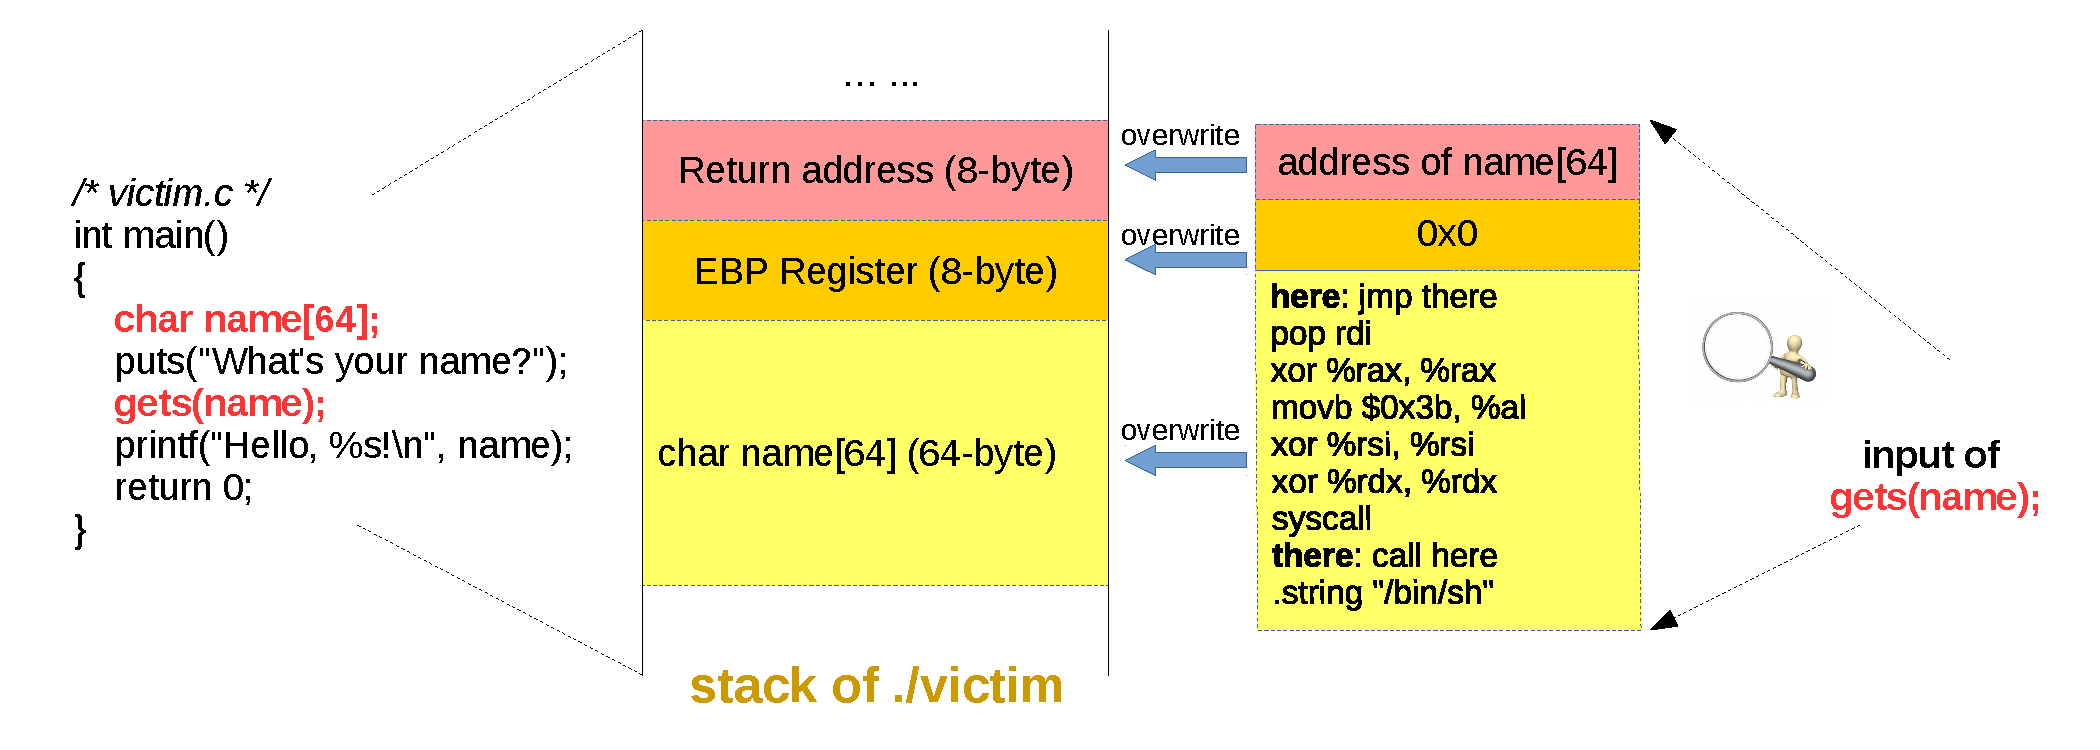
\includegraphics[width=1.0\linewidth]{figures/injection.pdf}
\end{figure}
\end{itemize}
\end{frame}

%------------------------------------------------

\section{Stack Smashing Mitigations}
\begin{frame}
\frametitle{Stack Smashing Mitigations}
\begin{itemize}
\item Stack Canary
	\begin{itemize}
		\item StackGuard: Automatic Adaptive Detectionand Prevention of Buffer-Overflow Attacks. USENIX Security 1998. \pause
		\item To disable via: \textit{\textcolor{red}{gcc -fno-stack-protector -o victim victim.c}} \pause
	\end{itemize}
\item DEP (Data Execution Prevention): W$\oplus$X (NX bit)
	\begin{itemize}
		\item Attackers are not able to execute any injected code!
		\item To disable via: \textit{\textcolor{red}{execstack -s victim}} \pause
	\end{itemize}
\item ASLR (Address Space Layout Randomization)
	\begin{itemize}
		\item Transparent runtime randomization for security. SRDS 2003. \pause
		\item To disable via: \textit{\textcolor{red}{setarch `arch` -R ./victim}}
		\item To disable via: \textit{\textcolor{red}{echo 0 $>$ /proc/sys/kernel/randomize\_va\_space}}
	\end{itemize}
\end{itemize}
\end{frame}

%------------------------------------------------

\section{Code Reuse Attack (1/2)}
\begin{frame}
\frametitle{Code Reuse Attack (1/2)}
\begin{itemize}
\item Gadgets: instruction sequence ended with "ret" instruction within existing program or libraries already present in memory
\item ROP (Return Oriented Programming): to perform arbitrary operations by chaining relavant gadgets to bypass DEP 
\begin{figure}
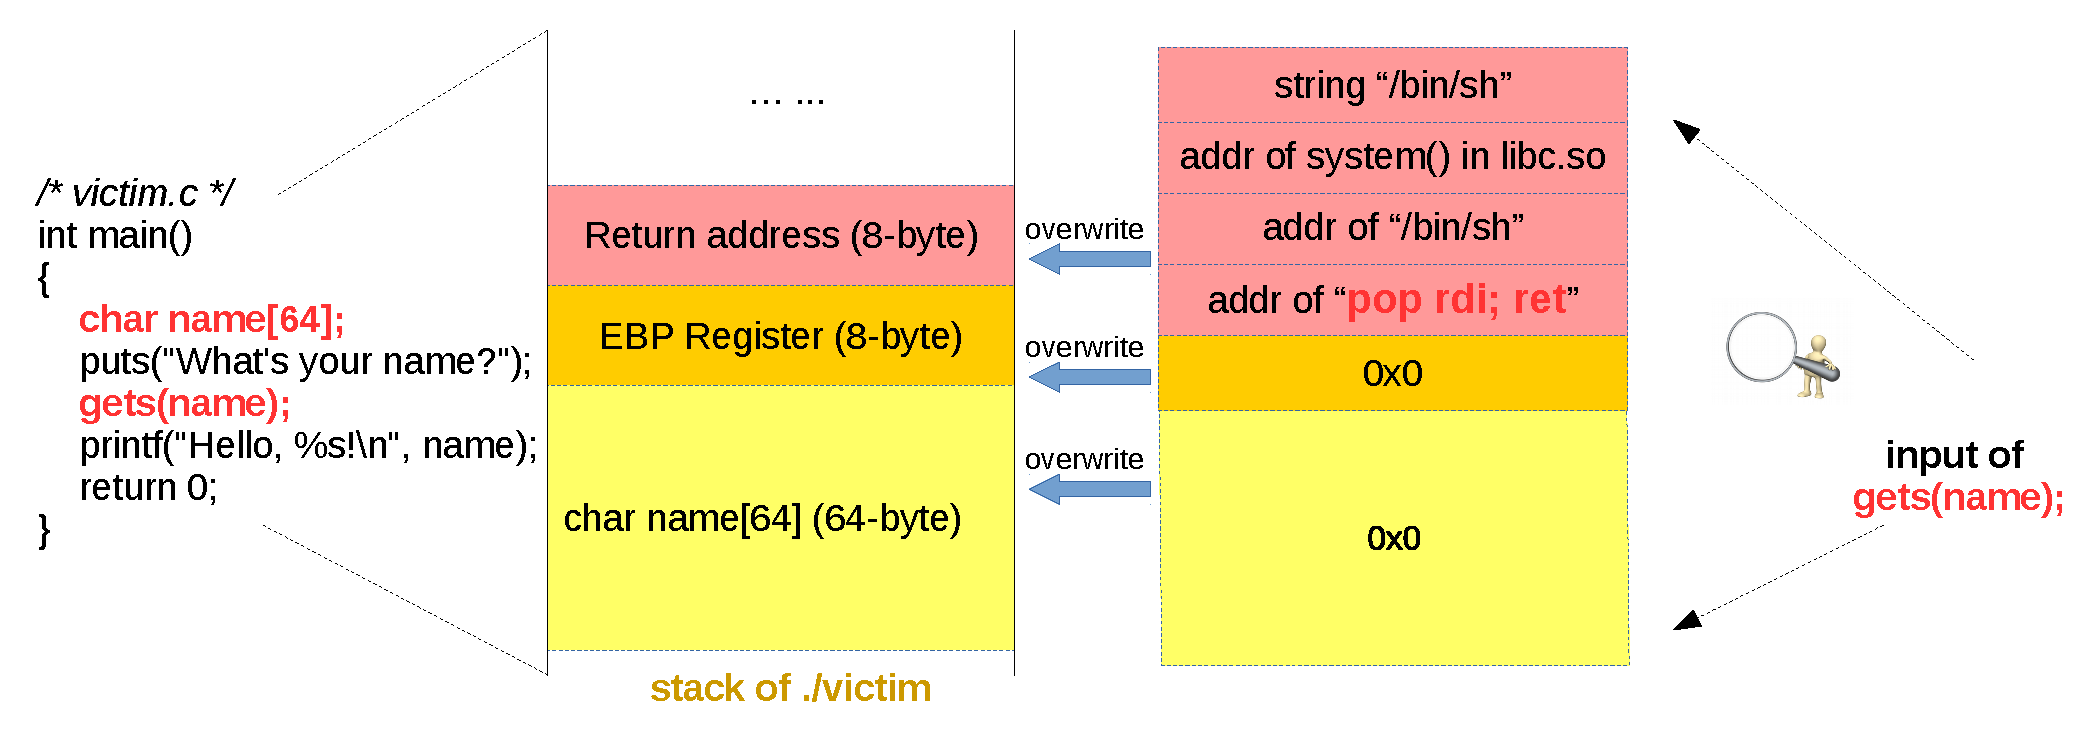
\includegraphics[width=1.0\linewidth]{figures/reuse.pdf}
\end{figure}
\end{itemize}
\end{frame}

%------------------------------------------------

\section{Code Reuse Attack (2/2)}
\begin{frame}
\frametitle{Code Reuse Attack (2/2)}
\begin{columns}[c]
\column{.40\textwidth}
\begin{figure}
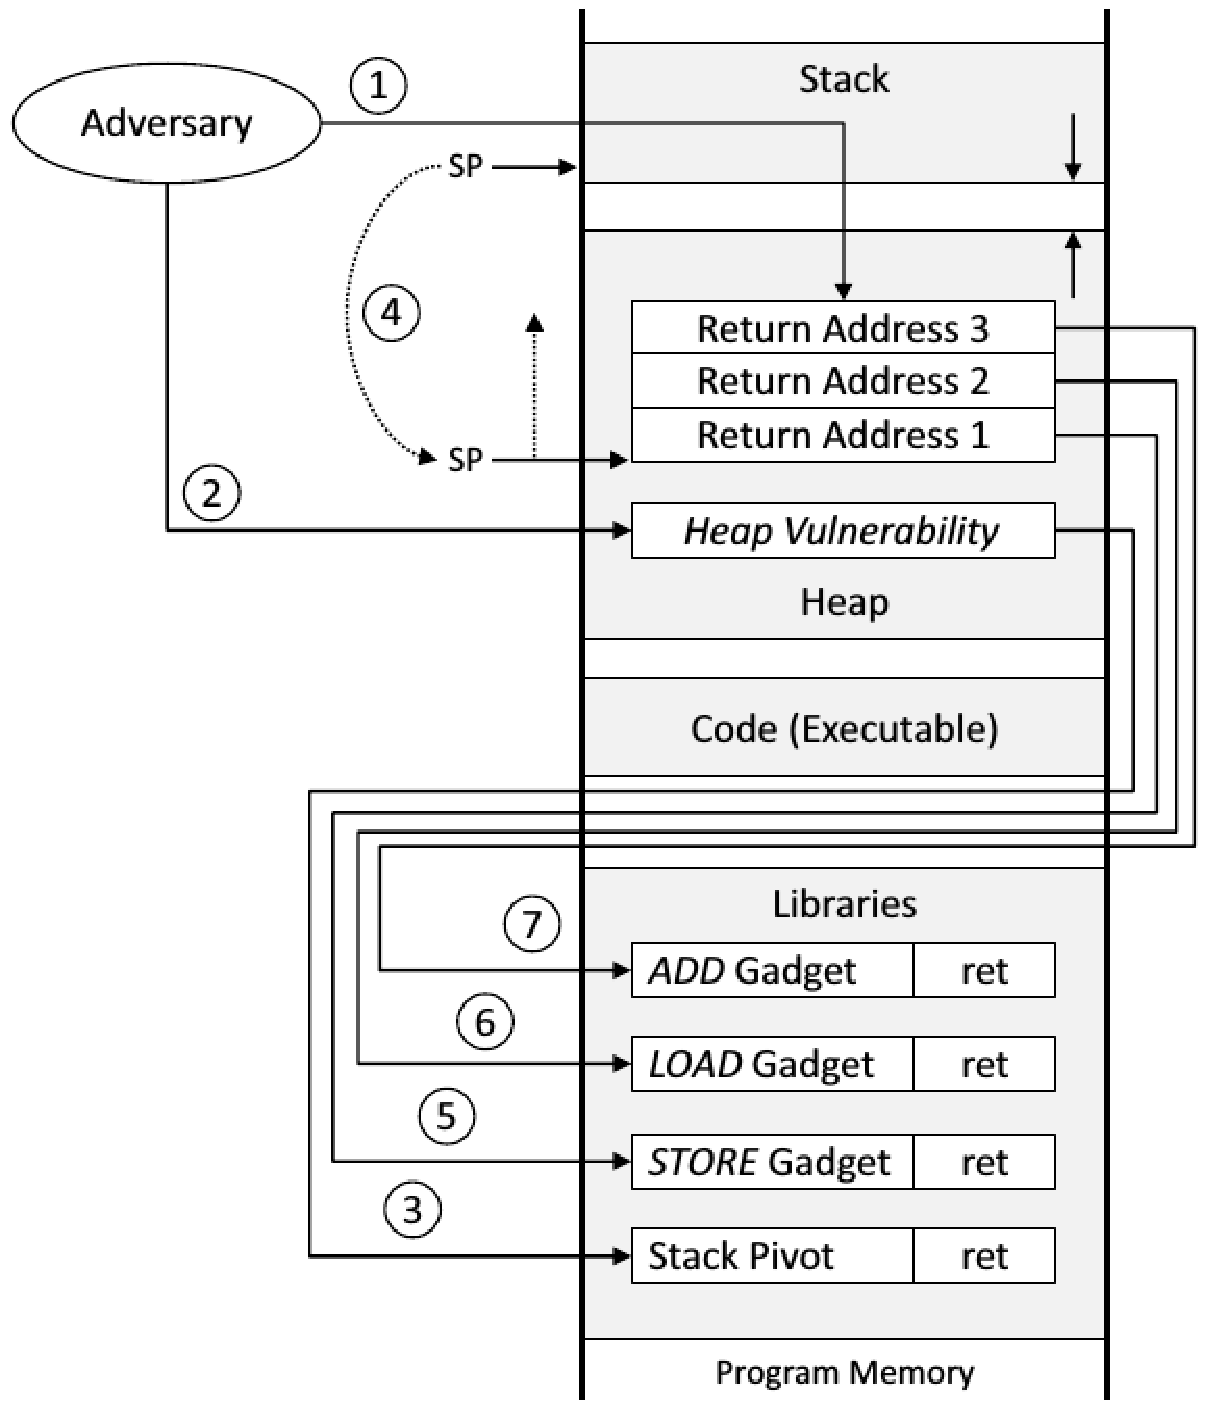
\includegraphics[width=1.0\linewidth]{figures/rop-sample.pdf}
\end{figure}
\column{.60\textwidth}
\begin{enumerate}
\visible<1->{\item inject ROP payload}
\visible<2->{\item hijack control flow}
\visible<3->{\item stack pivot sequences (e.g., mov \%eax, \%esp; ret)}
\visible<4->{\item "ret" redirects to ROP payload}
\visible<5->{\item ROP gadget and ret}
\visible<5->{\item ROP gadget and ret}
\visible<5->{\item ROP gadget and ret}
\end{enumerate}
\end{columns}
\end{frame}

%------------------------------------------------

\section{Fine-Grained Address Space Layout Randomization (ASLR)}
\begin{frame}
\frametitle{Fine-Grained Address Space Layout Randomization (ASLR)}
\begin{columns}[c]
\column{.60\textwidth}
\begin{itemize}
\item function order permutation
\item basic block order permutation
\item swap registers and replace instructions
\item instruction location randomization
\end{itemize}
\column{.40\textwidth}
\begin{figure}
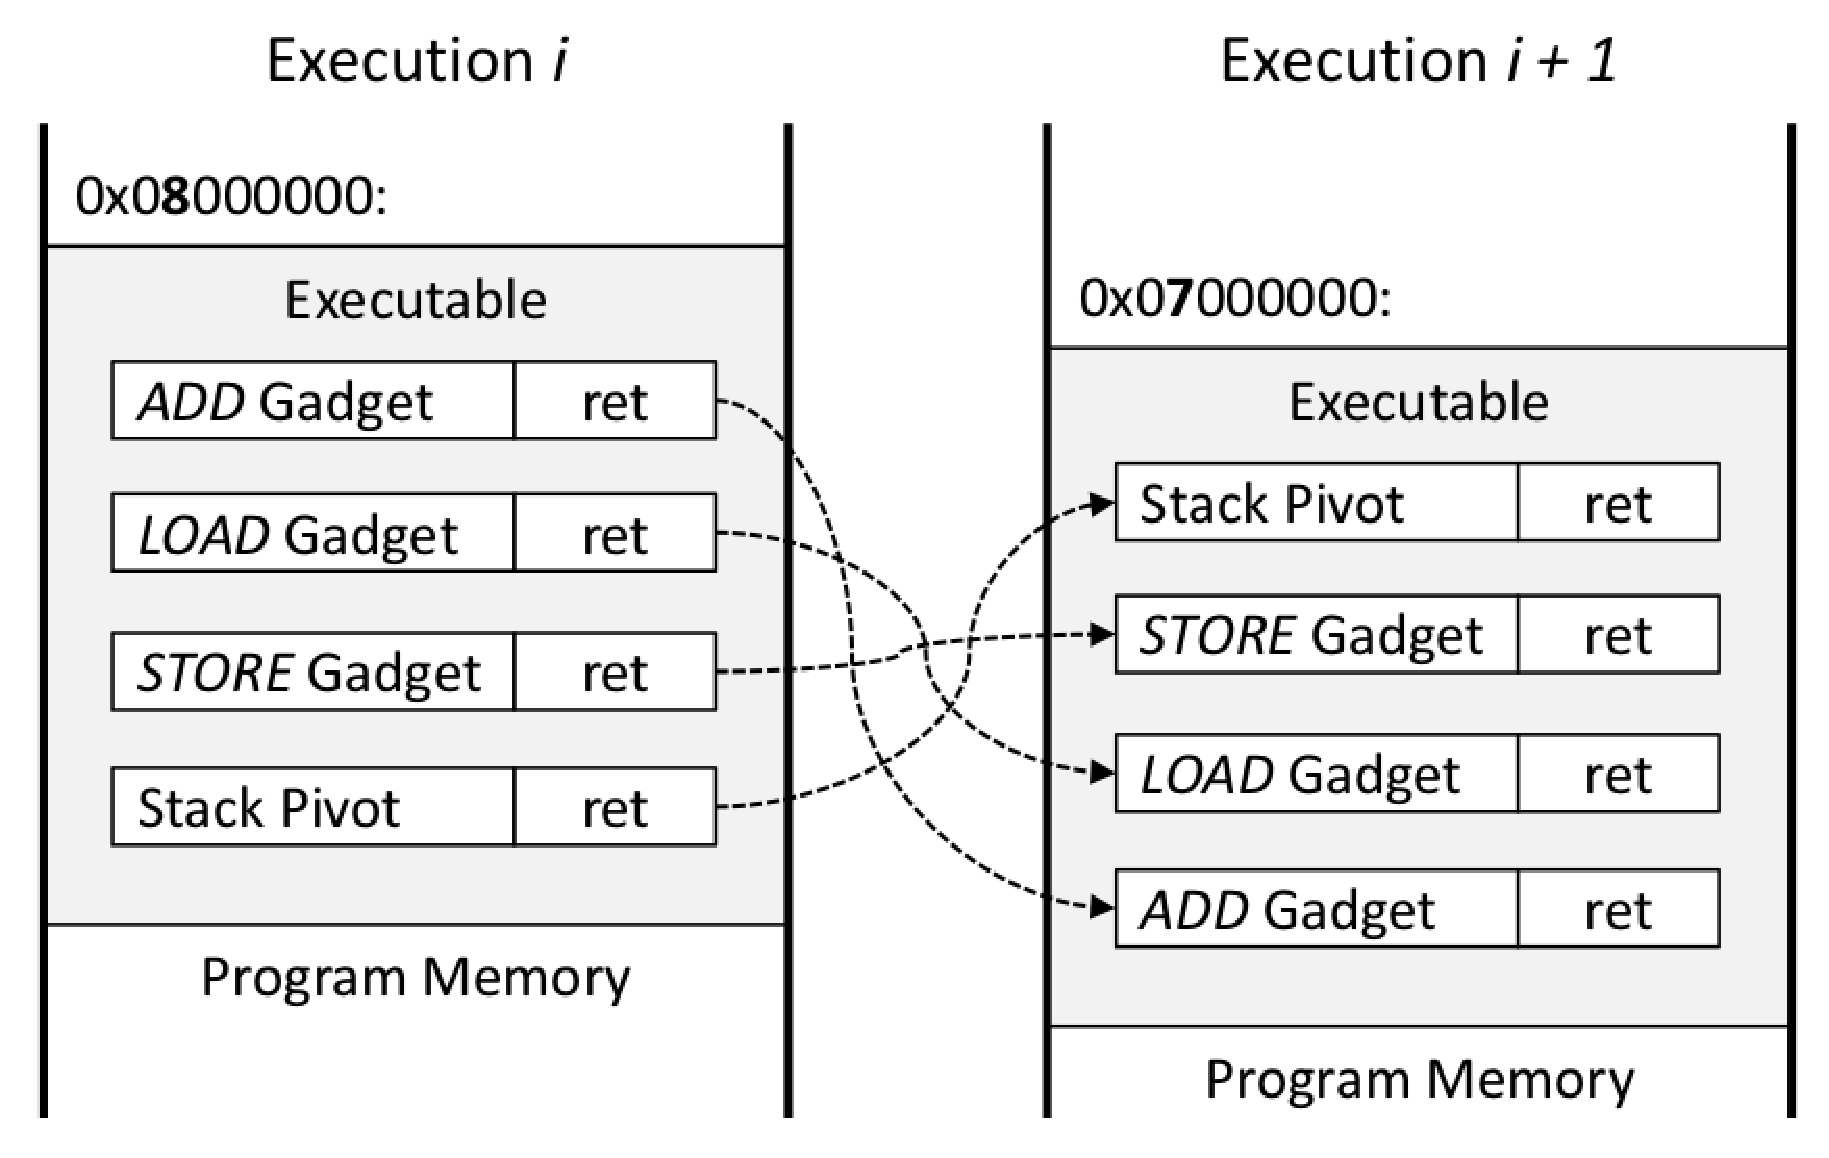
\includegraphics[width=1.0\linewidth]{figures/faslr.pdf}
\end{figure}
\end{columns}
\end{frame}

%------------------------------------------------

\section{Just-In-Time Return Oriented Programming Attack}
\begin{frame}
\frametitle{Just-In-Time Return Oriented Programming Attack}
\begin{itemize}
\item Just-In-Time Code Reuse: On the Effectiveness of Fine-Grained Address Space Layout Randomization. IEEE S\&P (Oakland) 2013
\end{itemize}	
\begin{columns}[c]
\column{.55\textwidth}
Thread Model Assumption
\begin{itemize}
\item Exercise a vulnerable entry point
\item Execute arbitrary malicious computations
\end{itemize}
\column{.45\textwidth}
\begin{figure}
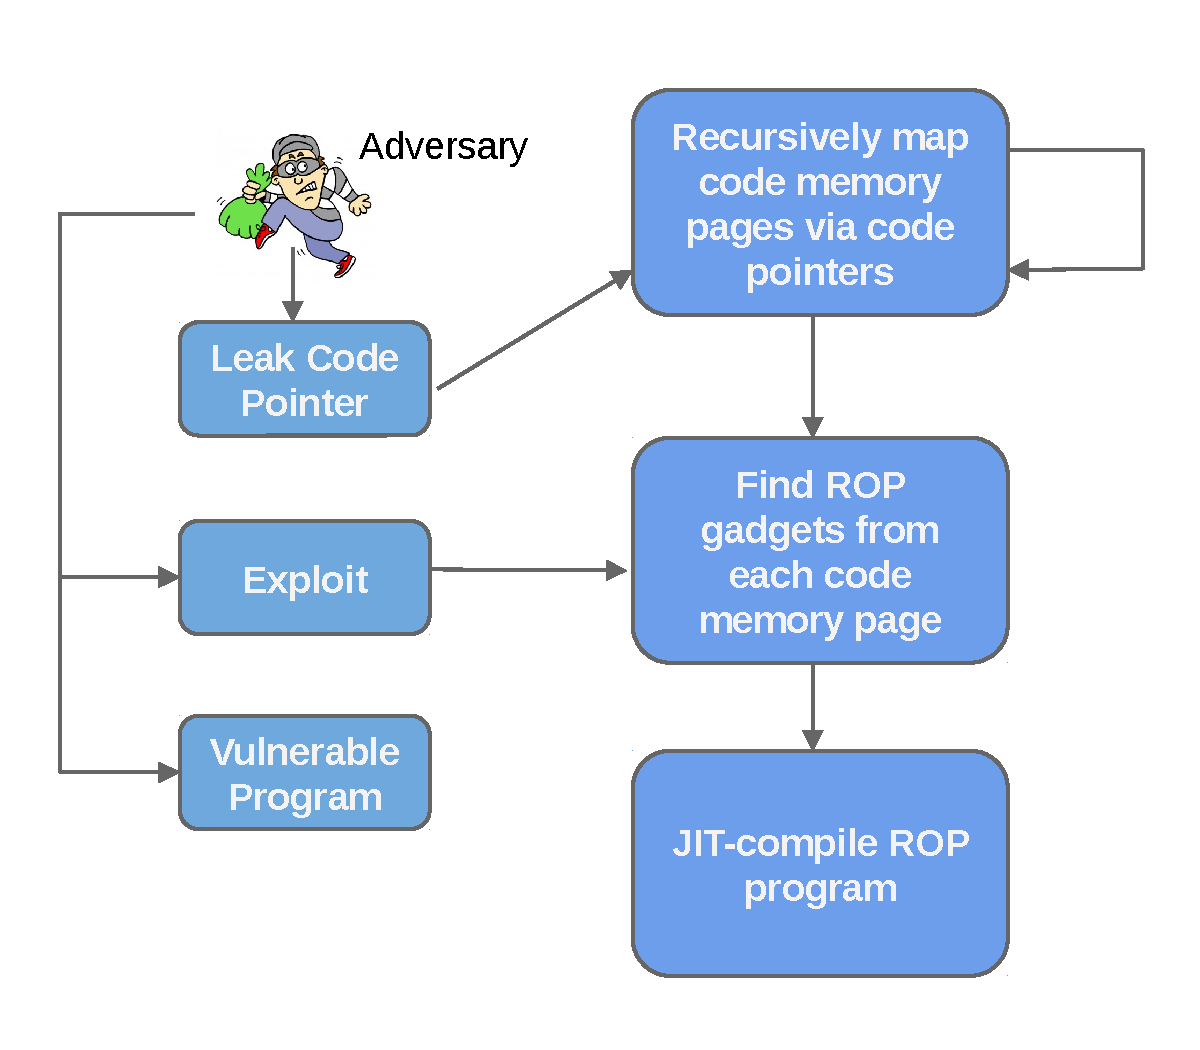
\includegraphics[width=1.0\linewidth]{figures/jitrop.pdf}
\end{figure}
\end{columns}

\end{frame}

%------------------------------------------------

\section{Memory Disclosure}
\begin{frame}
\frametitle{Memory Disclosure}
\begin{columns}[t]
\column{.5\textwidth}
\begin{center}
Direct Memory Disclosure
\begin{itemize}
\item read instructions in code page
\end{itemize}
\end{center}
\column{.5\textwidth}
\begin{center}
Indirect Memory Disclosure
\begin{itemize}
\item return address
\item function pointer
\item dynamic linking information
\item c++ vtable \& exception handler
\end{itemize}
\end{center}
\end{columns}
\begin{figure}
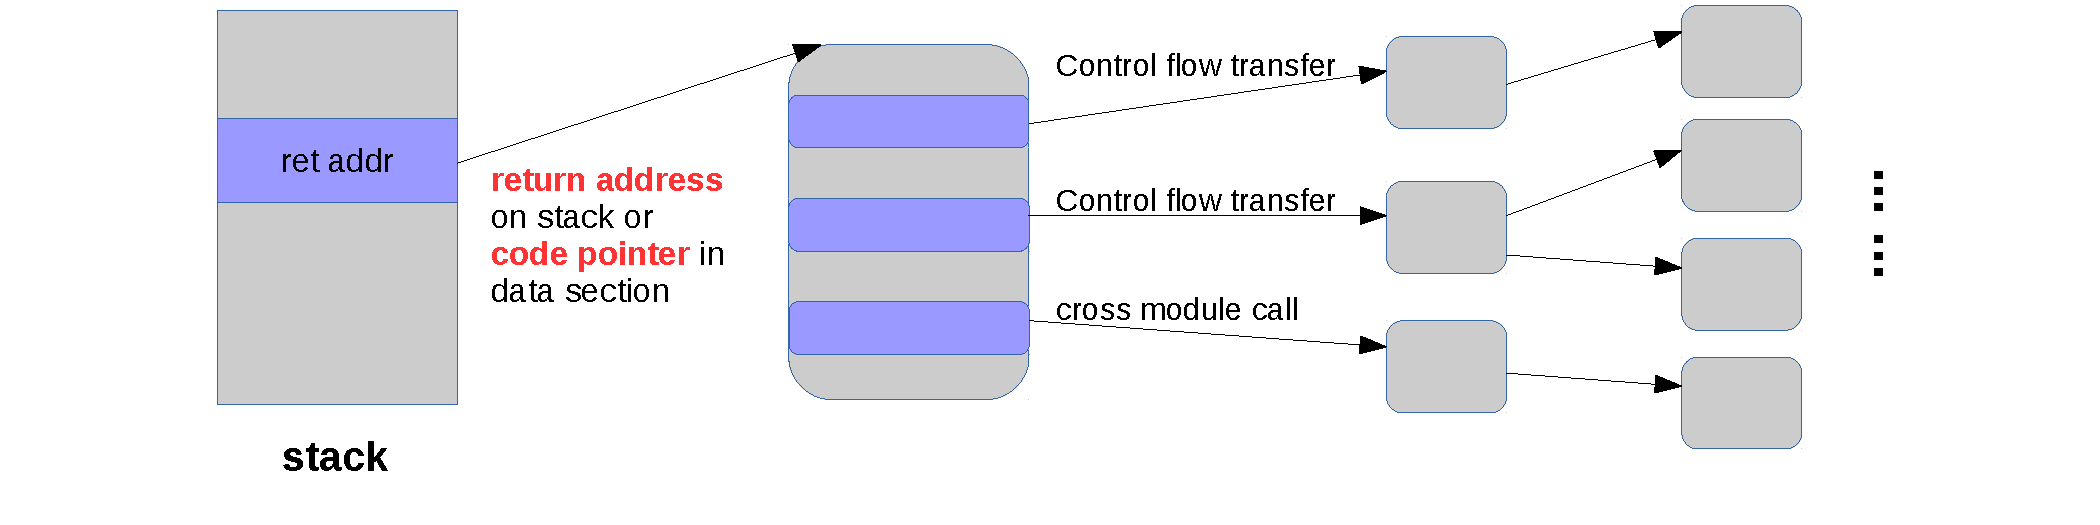
\includegraphics[width=1.0\linewidth]{figures/disclosure.pdf}
\end{figure}
\end{frame}

%------------------------------------------------

\section{Readactor 1/2}
\begin{frame}
\frametitle{Readactor 1/2}
\begin{columns}[c]
\column{.60\textwidth}
Readactor: Practical Code Randomization Resilient to Memory Disclosure. IEEE S \& P 2015
\begin{itemize}
\item Fine-grained code diversification via LLVM
\item Code and data separation via Intel EPT and LLVM
\item Code-pointer hiding via LLVM
\item Does not support COTS binary
\end{itemize}
\column{.40\textwidth}
\begin{figure}
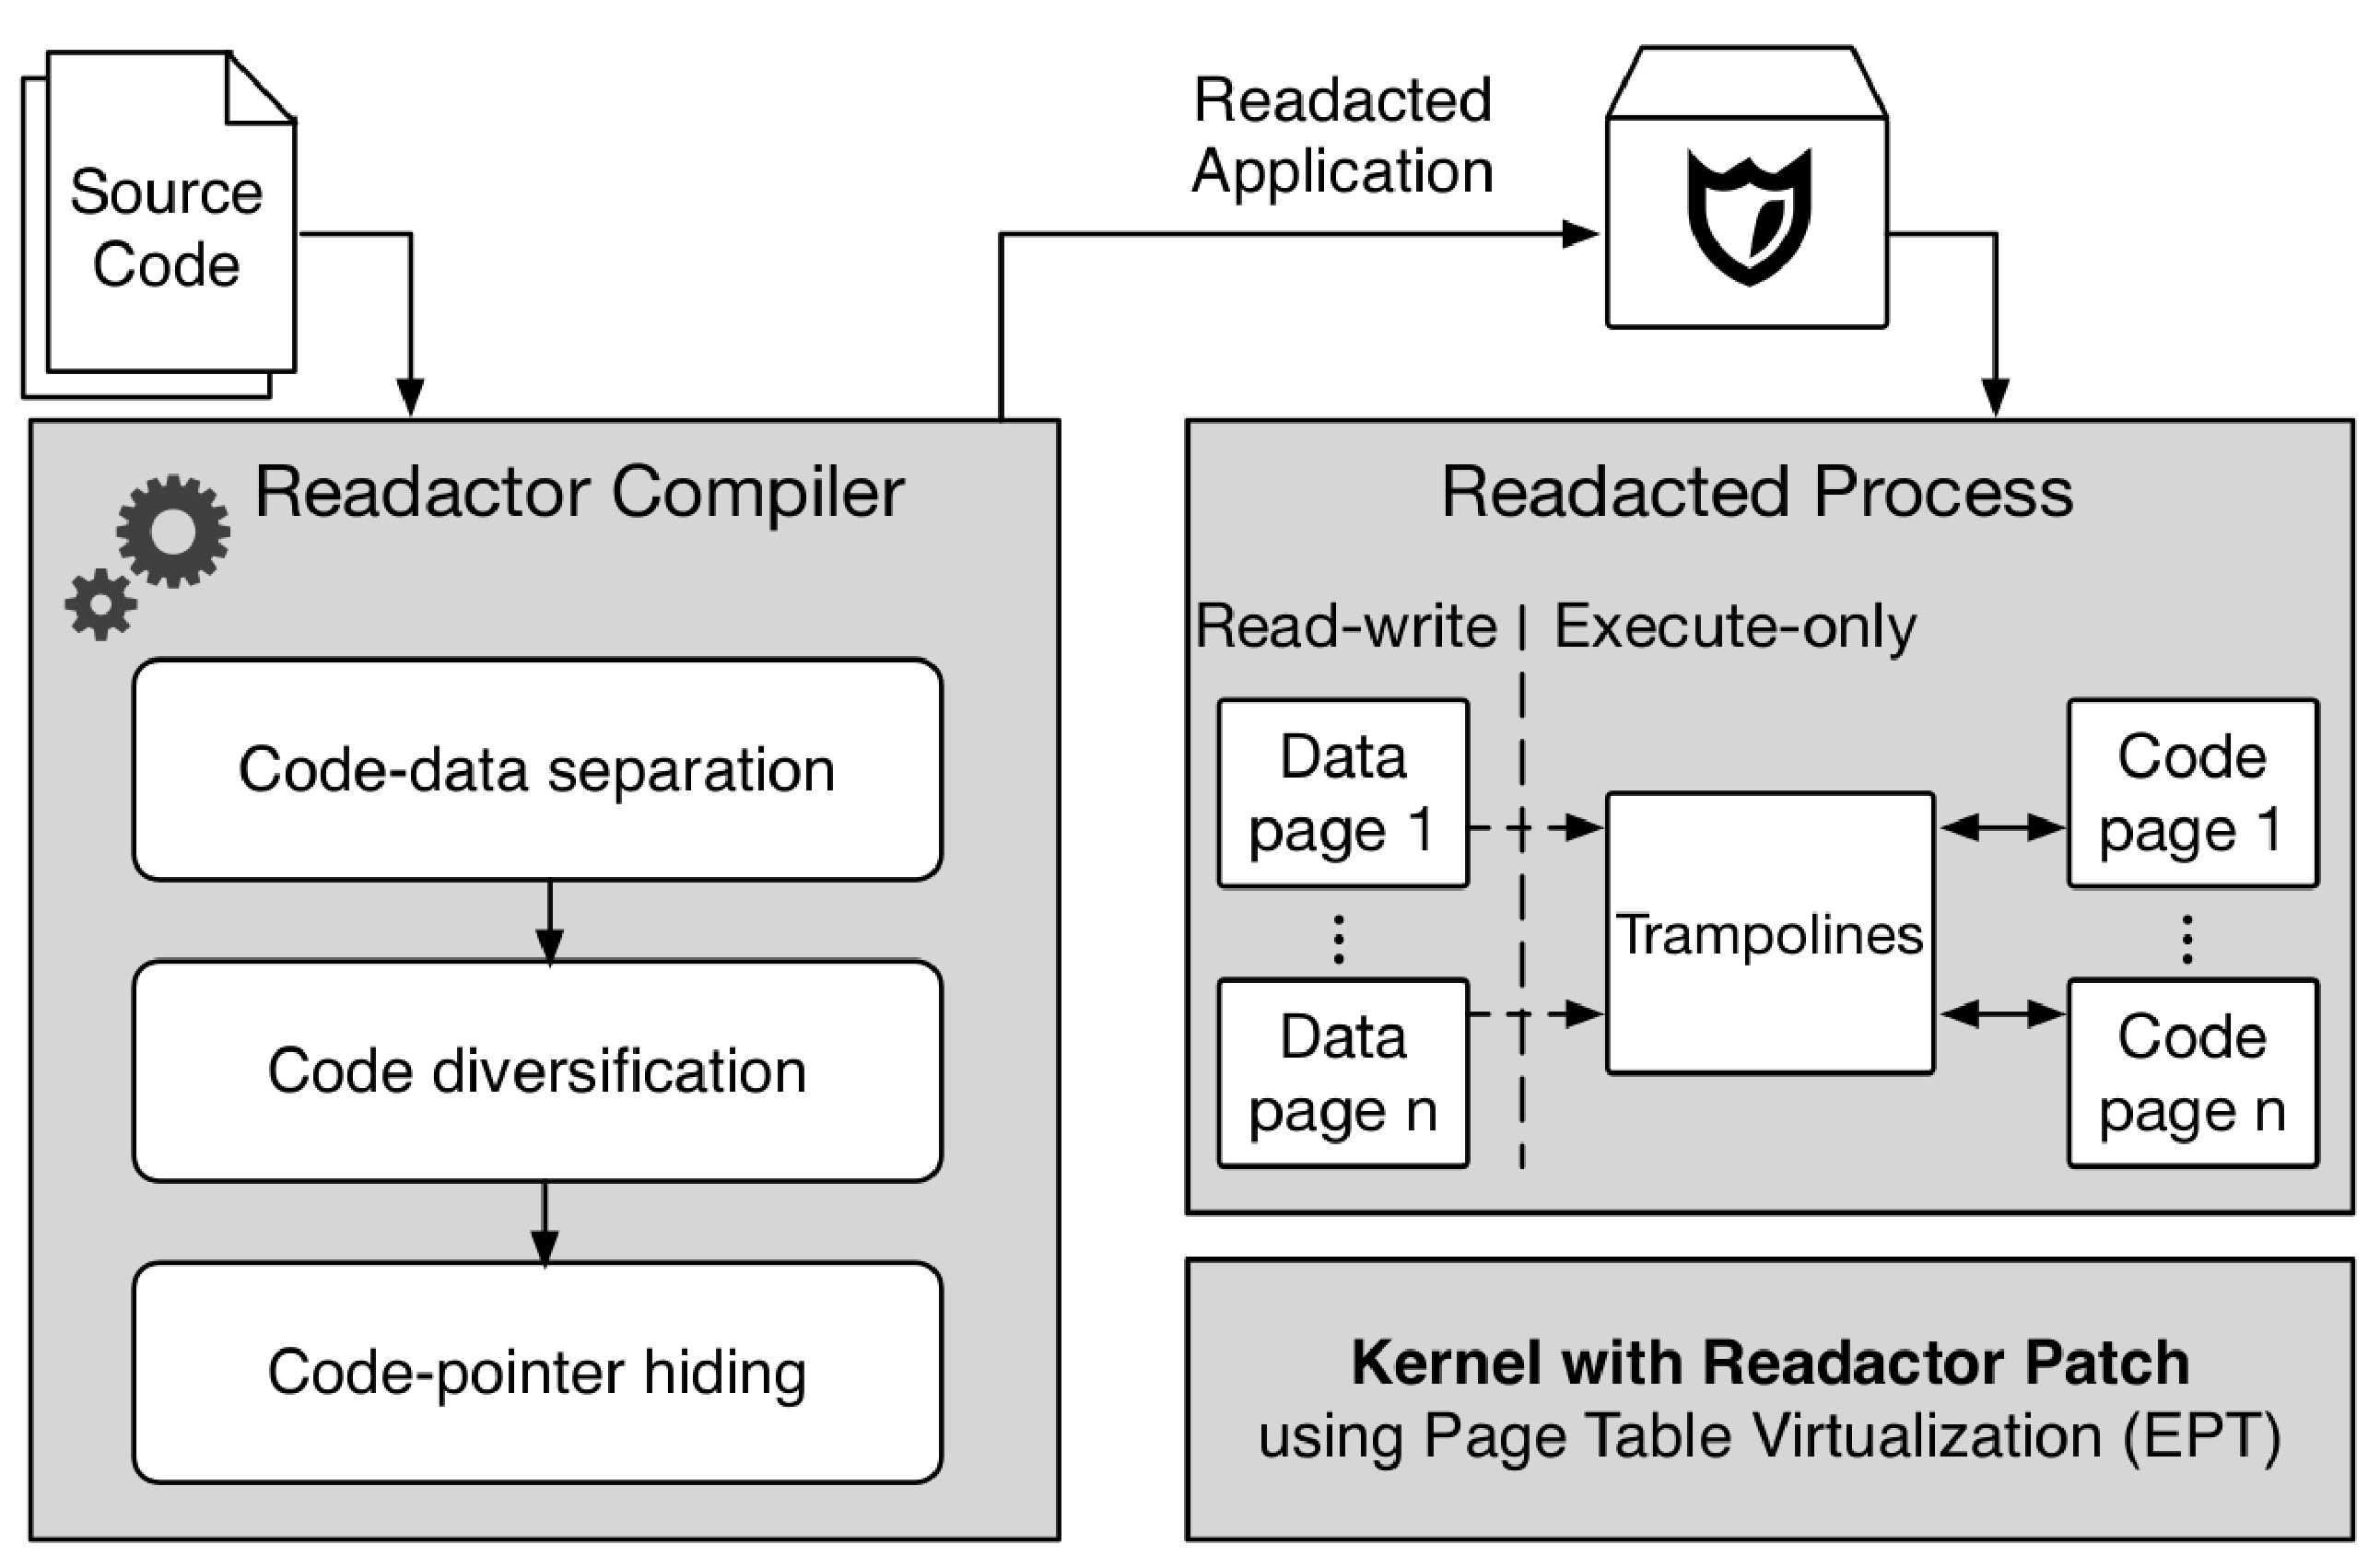
\includegraphics[width=1.0\linewidth]{figures/readactor-framework.pdf}
\end{figure}
\end{columns}
\end{frame}

%------------------------------------------------

\section{Readactor 2/2}
\begin{frame}
\frametitle{Readactor 2/2}
\begin{columns}[c]
\column{.30\textwidth}
\begin{figure}
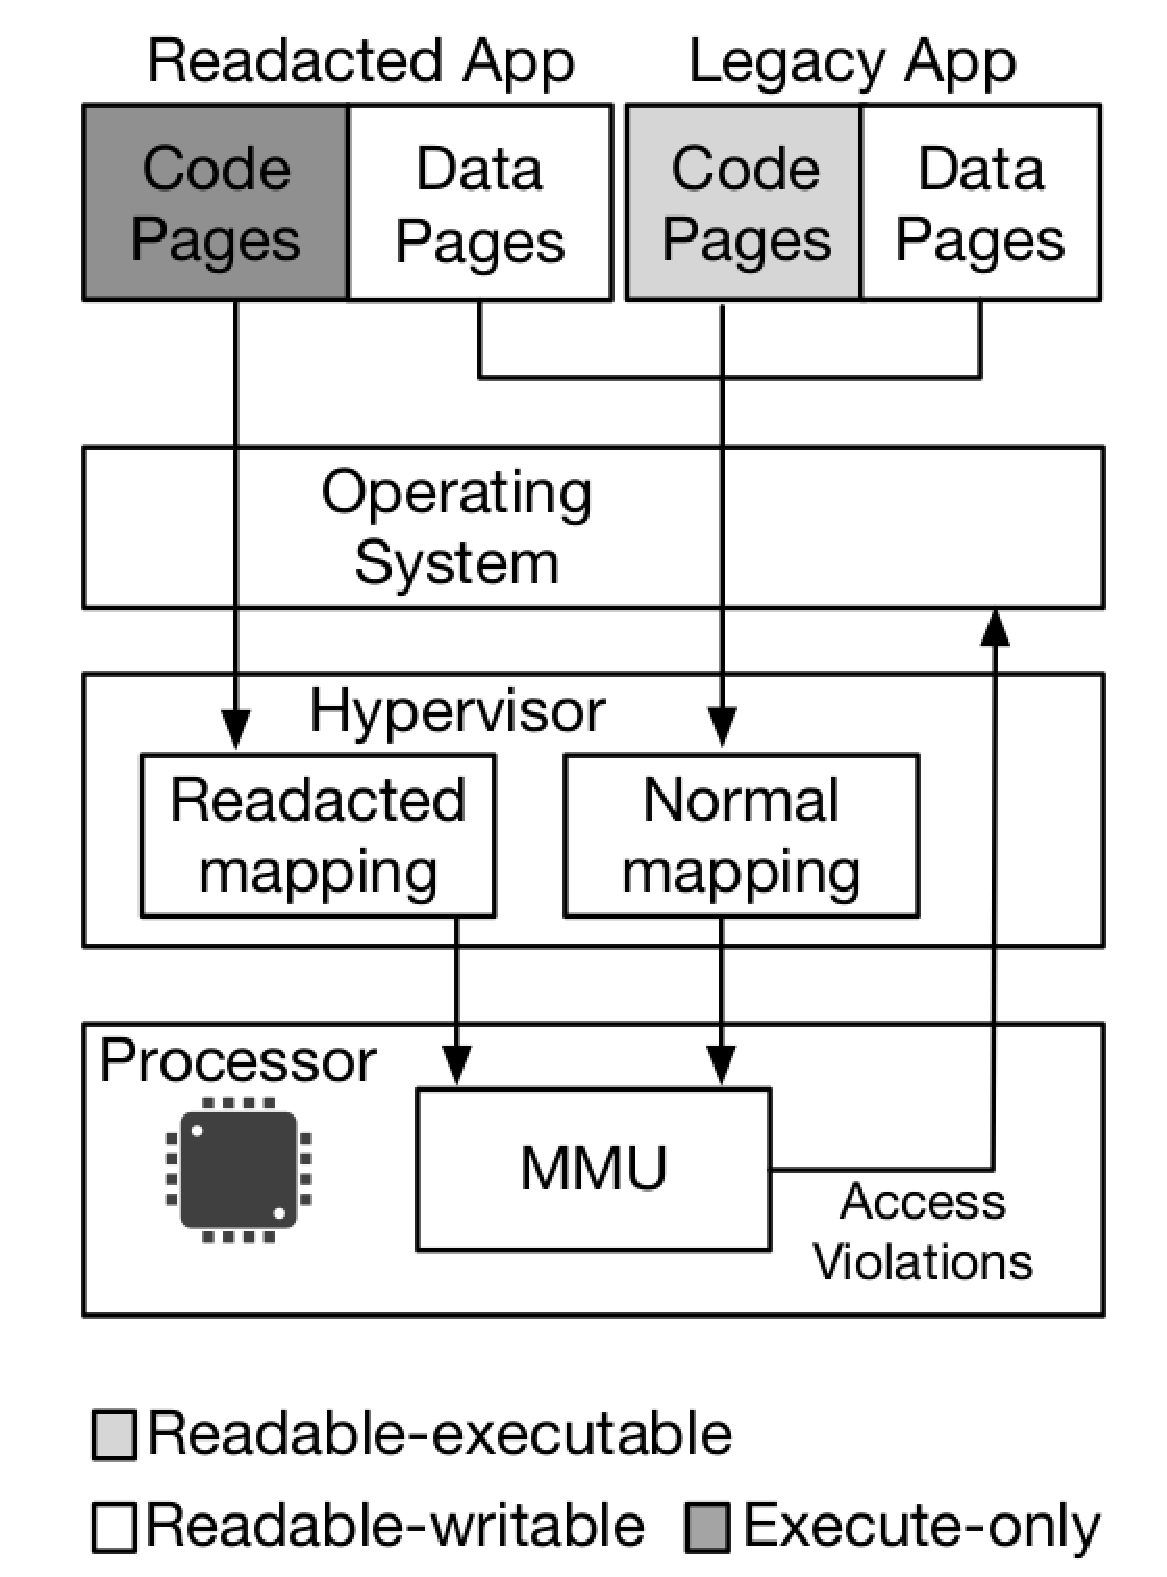
\includegraphics[width=1.0\linewidth]{figures/readactor-ept.pdf}
\end{figure} \pause
\column{.70\textwidth}
\begin{figure}
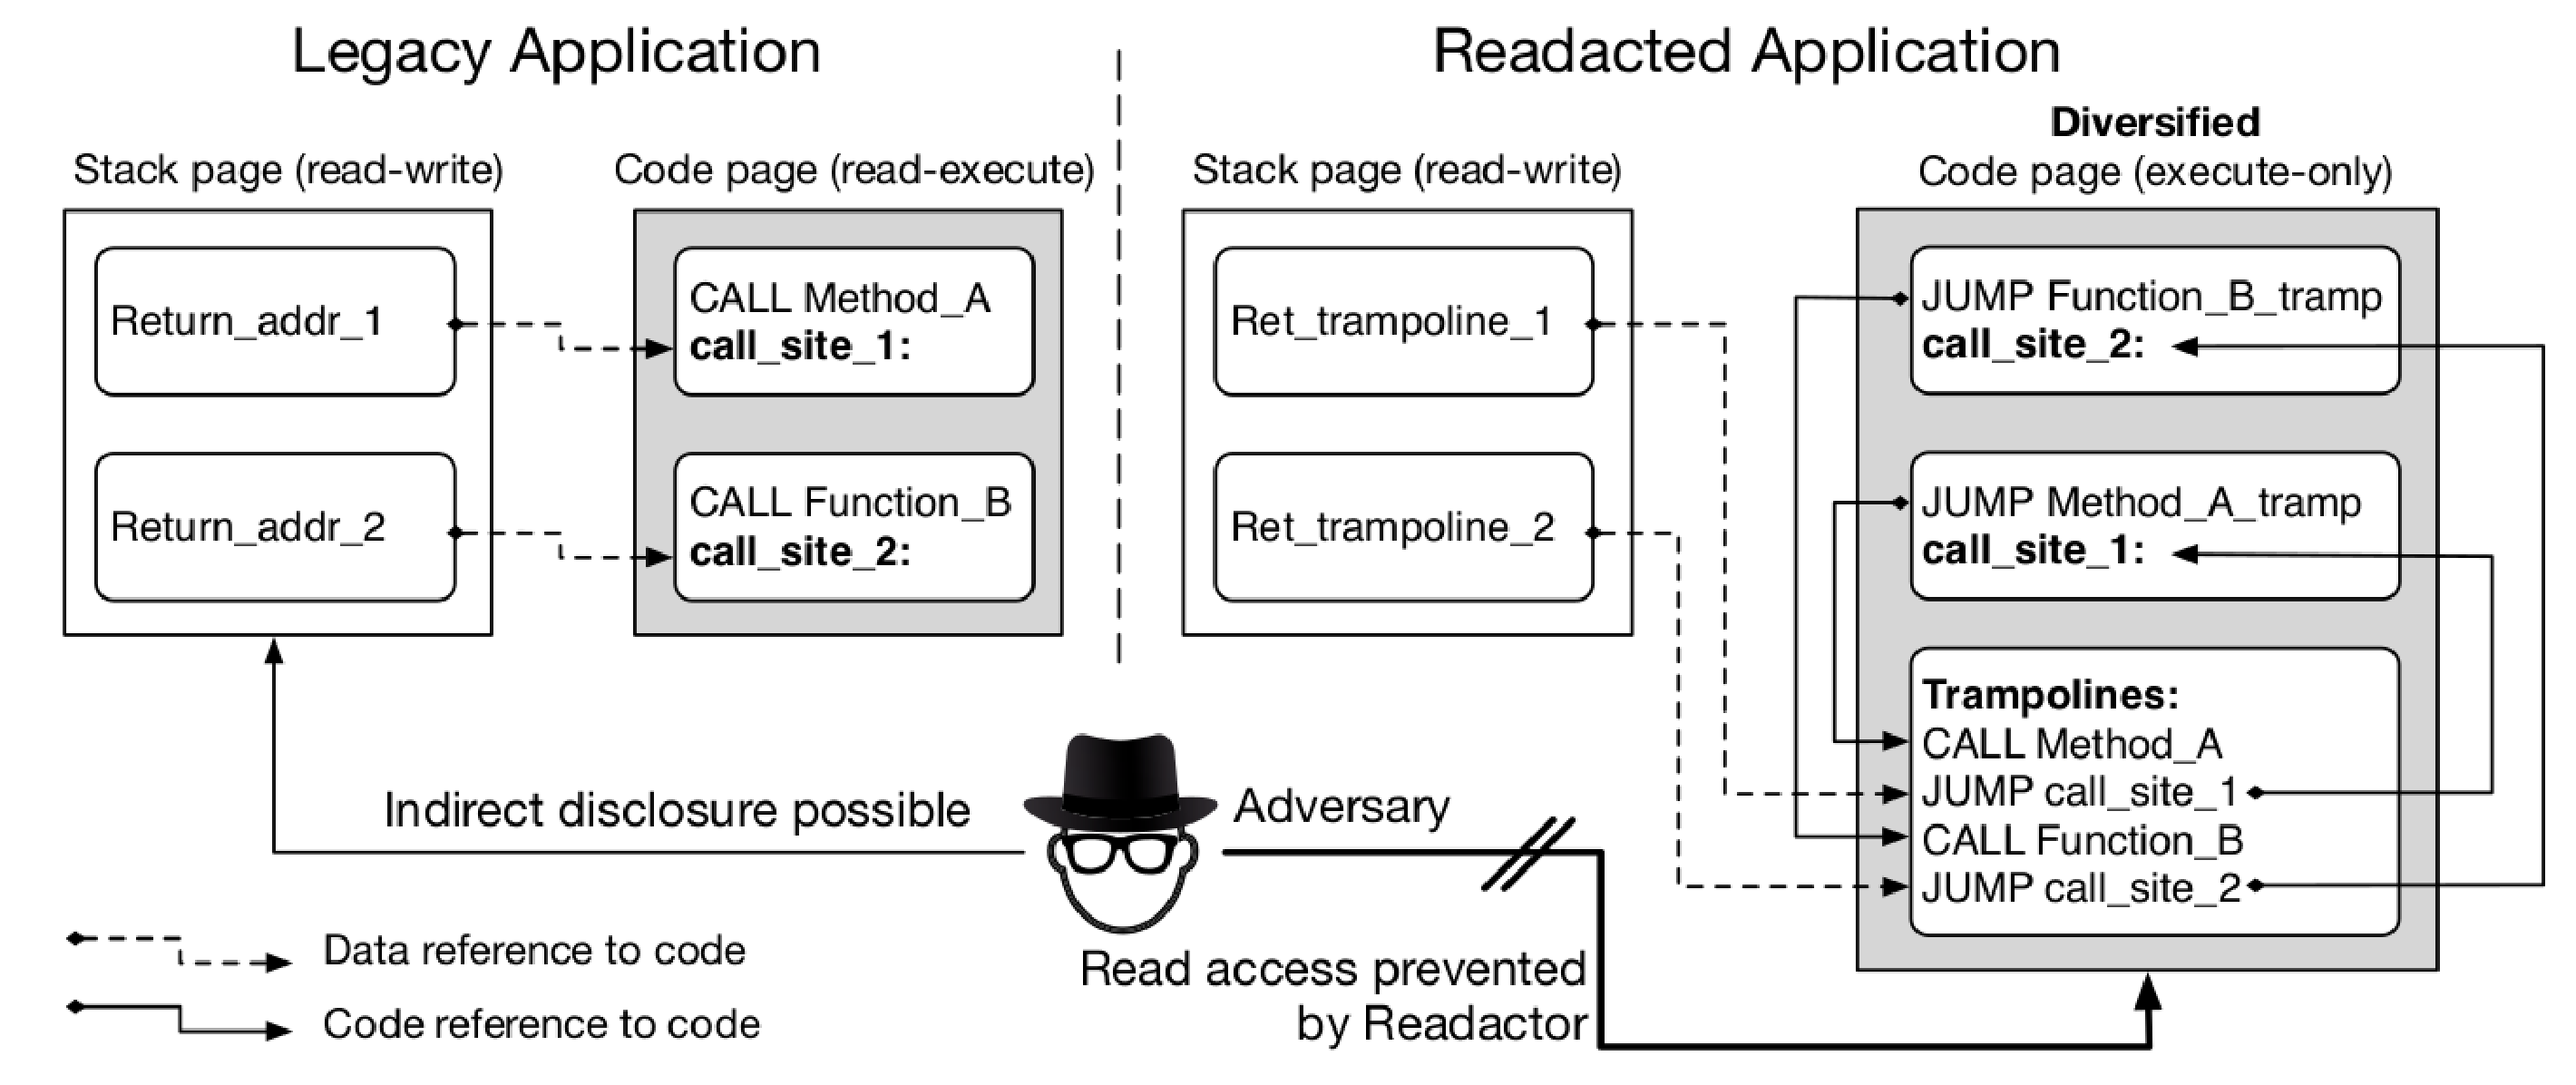
\includegraphics[width=1.0\linewidth]{figures/readactor-return.pdf}
\end{figure}
\end{columns}
\end{frame}

%------------------------------------------------

\section{New and Hard Problem}
\begin{frame}
\frametitle{New and Hard Problem}
\begin{figure}
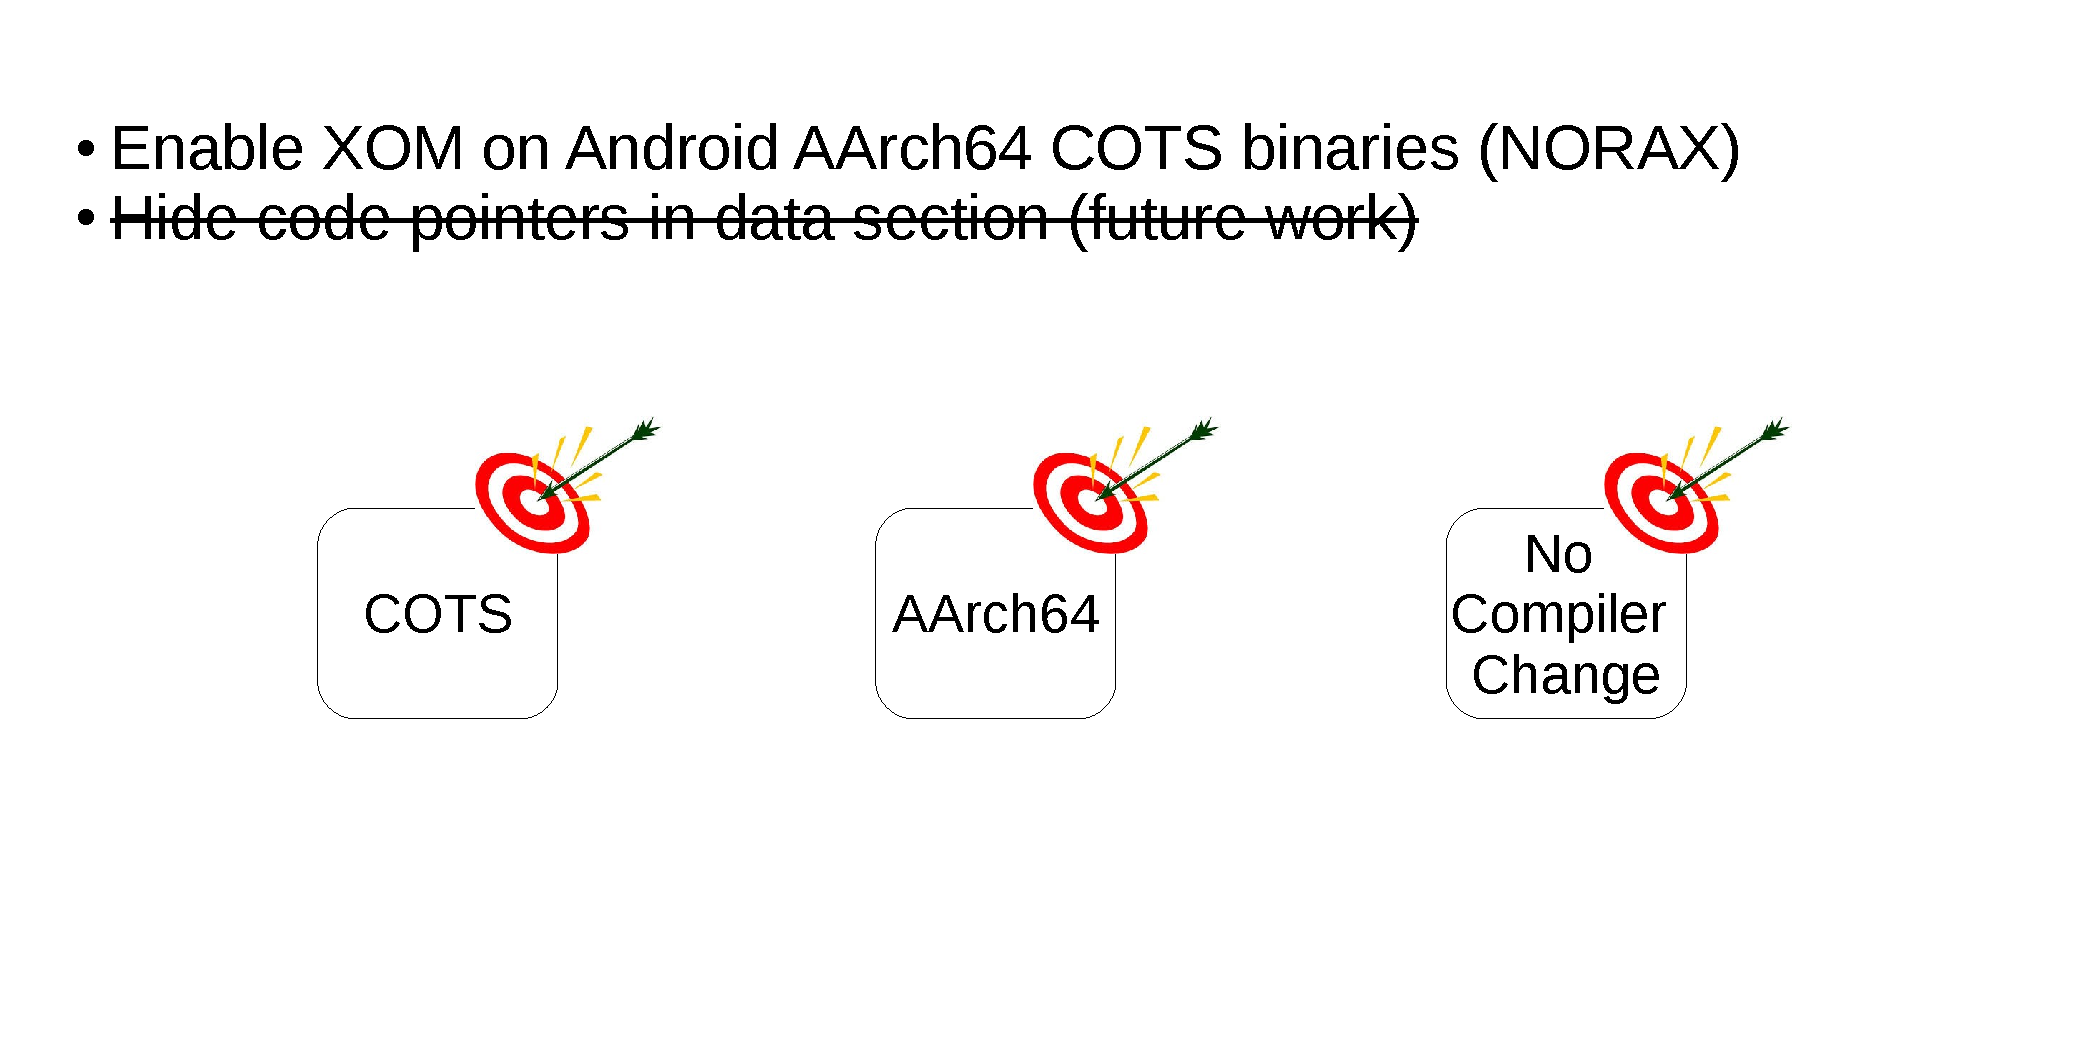
\includegraphics[width=1.0\linewidth]{figures/problem.pdf}
\end{figure}
\end{frame}

%------------------------------------------------


\section{COTS Binary - Commercial Off-The-Shelf}
\begin{frame}
\frametitle{COTS Binary - Commercial Off-The-Shelf}
\begin{itemize}
\item $\#$ aarch64-linux-gnu-strip $<$binary$>$
\item without symbol information
\end{itemize}
\begin{figure}
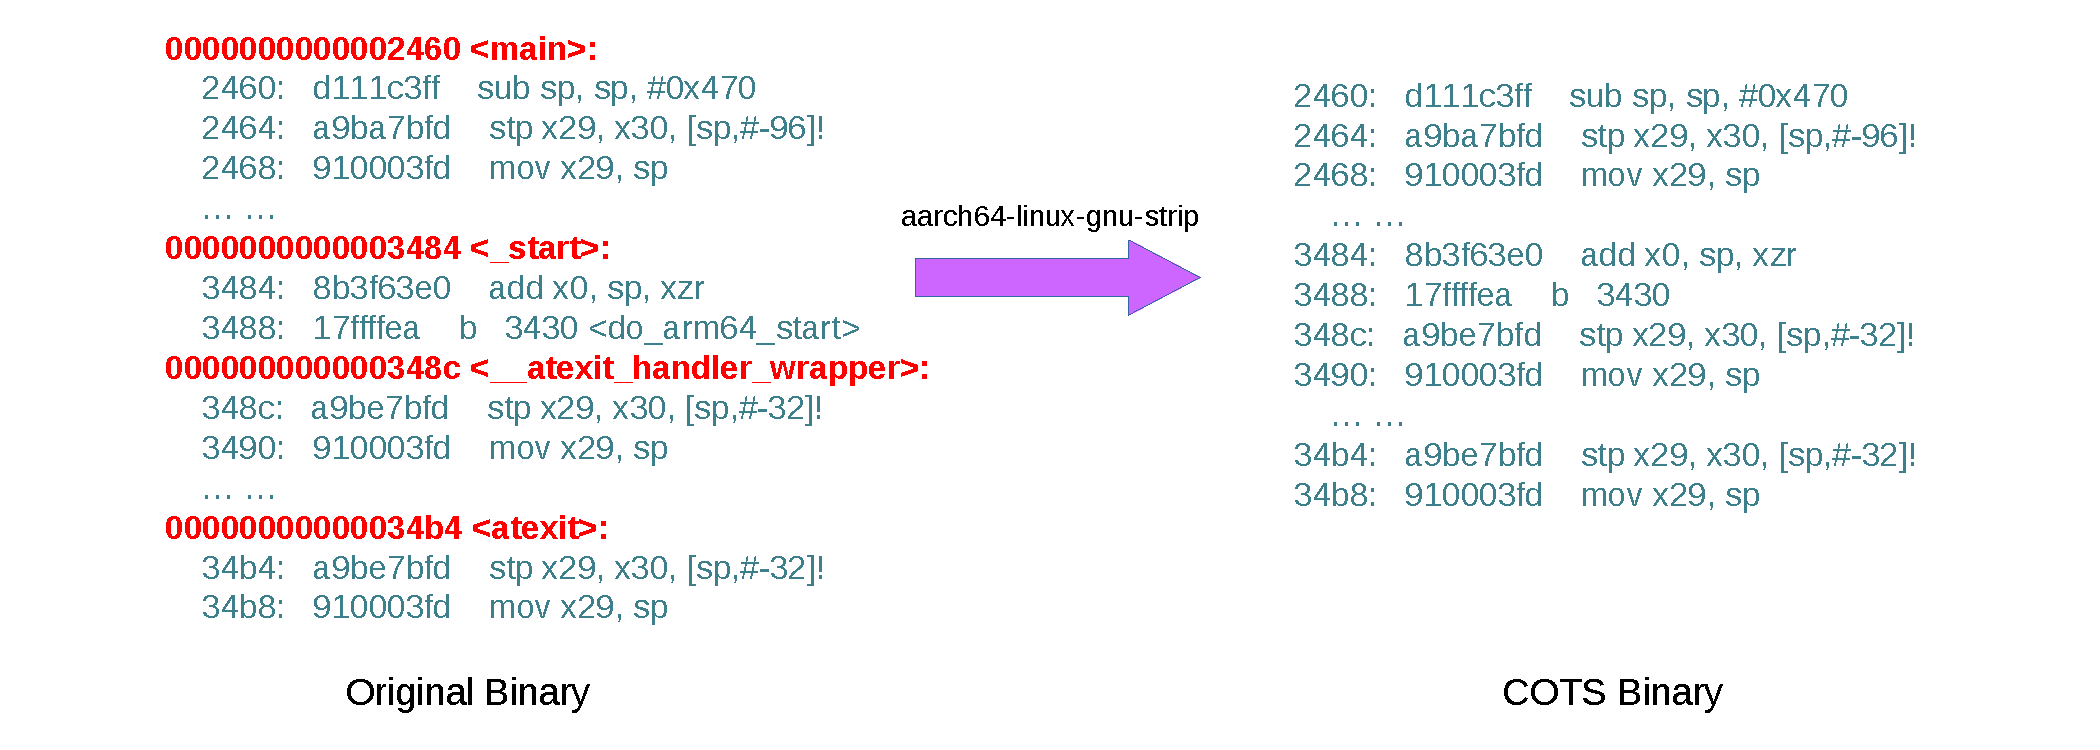
\includegraphics[width=1.0\linewidth]{figures/cots.pdf}
\end{figure}
\end{frame}

%------------------------------------------------

\section{ELF - Linking vs. Execution}
\begin{frame}
\frametitle{ELF - Linking vs. Execution}
\begin{columns}[c]
\column{.55\textwidth}
\begin{itemize}
\item segments sample
	\begin{itemize}
		\item INTERP
		\item LOAD
		\item DYNAMIC
	\end{itemize}
\item sections sample
	\begin{itemize}
		\item .interp
		\item .dynsym, .dynamic
		\item .rela.dyn, .rela.plt, .got.plt, .got
		\item .plt, .text
		\item .data, .rodata, .bss
	\end{itemize}
\item manuals
	\begin{itemize}
		\item Executable and Linkable Format (ELF)
		\item ELF for the ARM Architecture
		\item ELF for the ARM 64-bit Architecture (AArch64)
	\end{itemize}
\end{itemize}
\column{.45\textwidth}
\begin{figure}
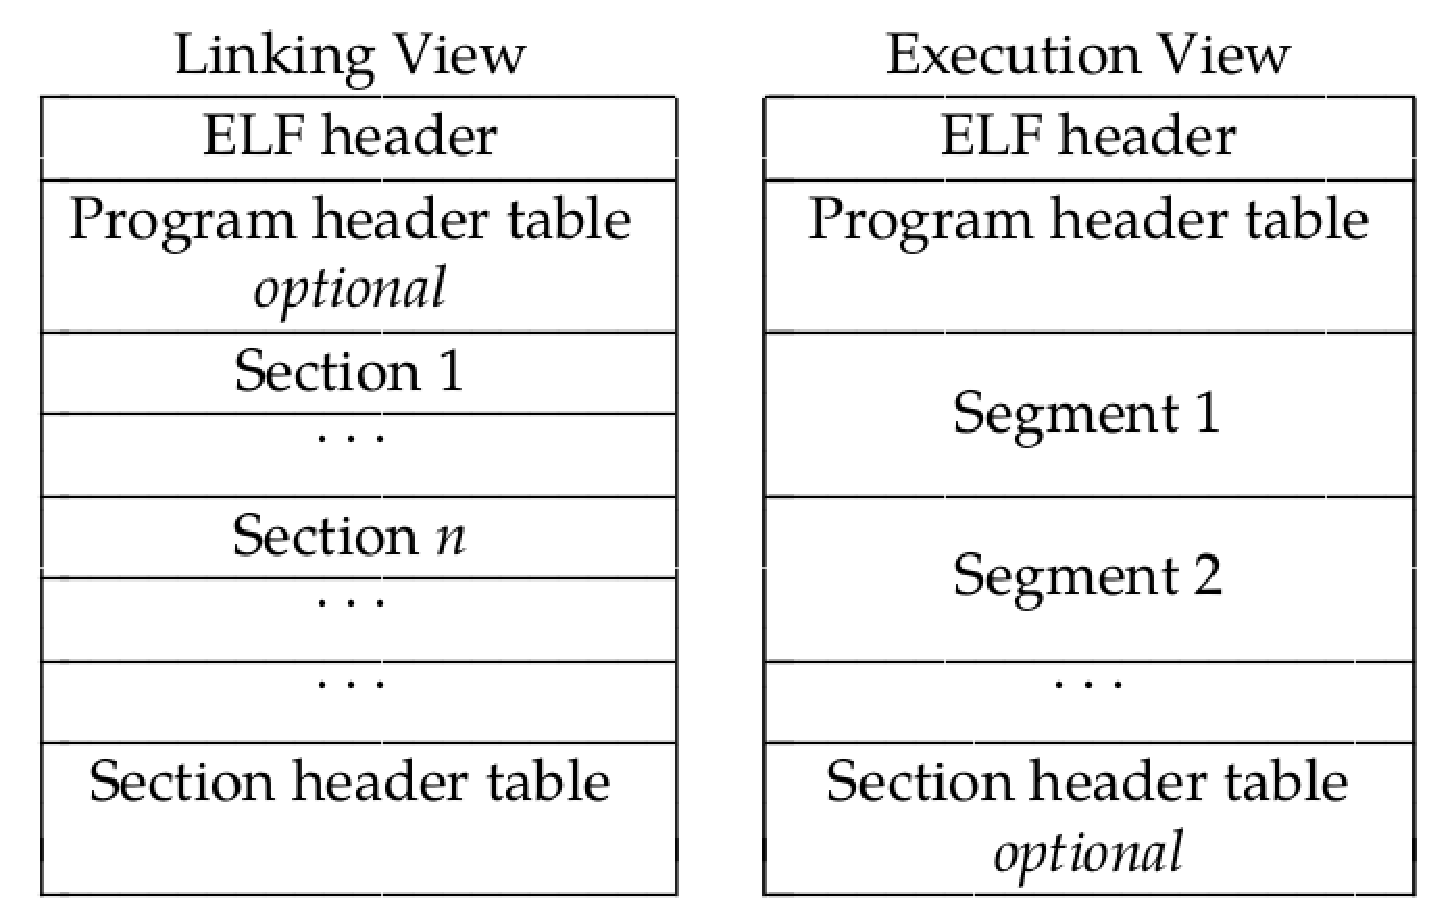
\includegraphics[width=1.0\linewidth]{figures/elf.pdf}
\end{figure}
\end{columns}
\end{frame}

%------------------------------------------------

\section{ELF - load executable ELF}
\begin{frame}
\frametitle{ELF - load executable ELF}
\begin{enumerate}
\visible<1->{\item user space loads executable binary via exec system call}
\visible<2->{\item kernel loads executable binary and dynamic linker into memory}
\visible<3->{\item dynamic linker performs linking jobs while loading all prerequisite libraries (android is without lazy address resolution)}
\visible<4->{\item start the executable binary}
\visible<5->{\item resolve dynamic symbol on-demand by linker}
\end{enumerate}
\end{frame}

%------------------------------------------------

\section{ELF - resolve dynamic symbol}
\begin{frame}
\frametitle{ELF - resolve dynamic symbol}
Suppose ./test calls function puts() belong to libc (lazy address resolution):
\begin{enumerate}
\visible<1->{\item ./test calls puts@plt belong to plt section}
\visible<2->{\item puts@plt redirects to puts in got.plt which points to corresponding handler in ld}
\visible<3->{\item ld calculates the hash of symbol name (puts), traverses each libraries and searches in buckets of gnu.hash with the hash value to identify the index of puts() in dynsym section}
\visible<4->{\item Once entry of puts in dynsym is identified, the address of puts would be written to got.plt with the help of binary's rela.plt}
\end{enumerate}
\end{frame}

%------------------------------------------------

\section{AArch64}
\begin{frame}
\frametitle{AArch64}
\begin{columns}[c]
\column{.55\textwidth}
\begin{itemize}
\visible<1->{\item instructions: 4-byte aligned and fixed size}
\visible<2->{\item mode: user (EL0), kernel (EL1), hypervisor (EL2) and secure monitor (EL3)}
\visible<3->{\item registers: X0-X30 (X29 is FP, X30 is LR), SP (PC is not accessible)}
\visible<4->{\item branch: B, BL (Branch with Link), BLR (Branch with Link to Register), BR (Branch to Register), B.cond}
\visible<5->{\item memory load: ADR, ADRP, LDR}
\visible<6->{\item other: ARM Architecture Reference Manual: ARMv8, for ARMv8-A architecture profile}
\visible<7->{\item since Android 5.0 (Lolopop), non-PIE loading is no longer supported}
\end{itemize}
\column{.45\textwidth}
\begin{figure}
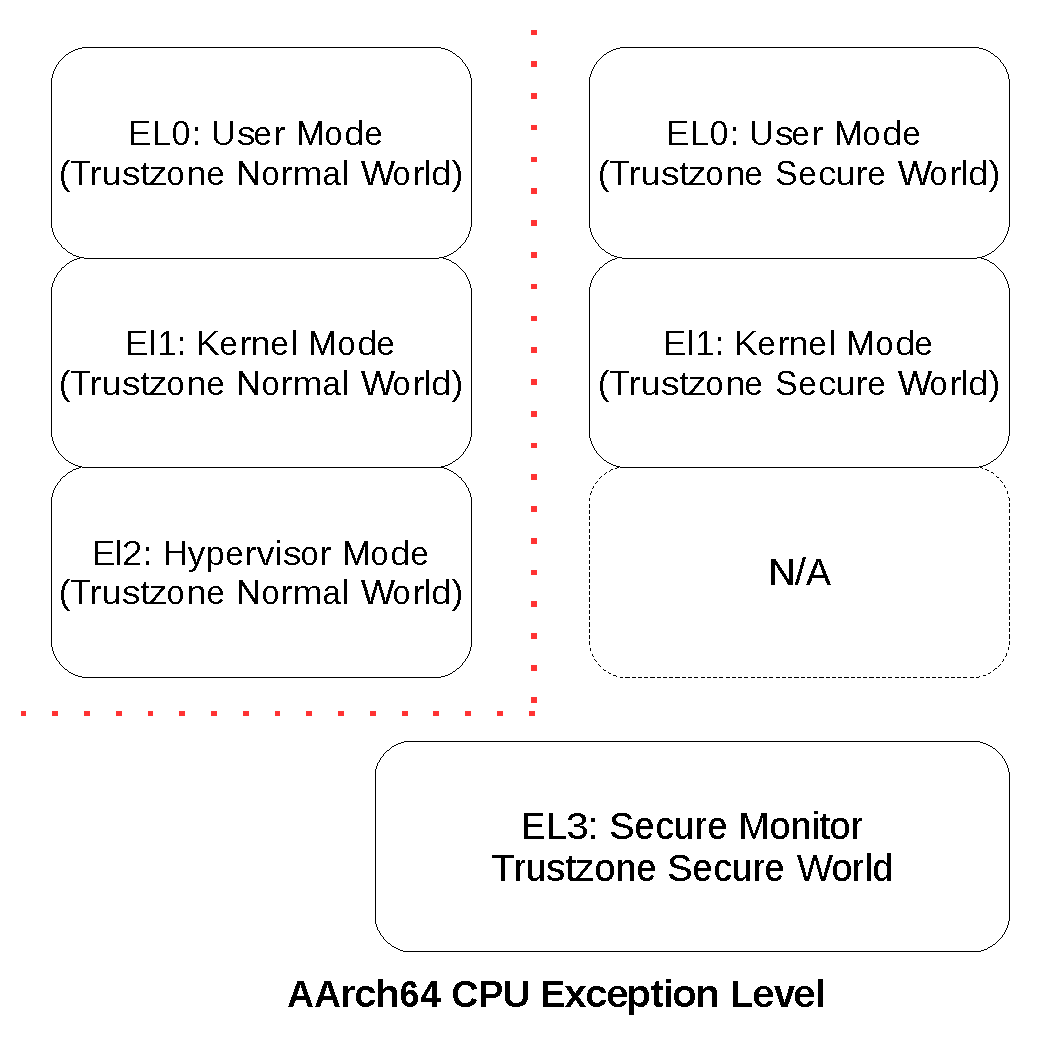
\includegraphics[width=1.0\linewidth]{figures/aarch64.pdf}
\end{figure}
\end{columns}
\end{frame}

%------------------------------------------------

\section{NORAX}
\begin{frame}
\frametitle{NORAX}
\begin{center}
{\huge{NORAX: Enabling Execute-Only Memory for COTS Binaries on AArch64}}
\\~\\

$^{\ast}Yaohui Chen, ^{\ast}Dongli Zhang, ^{\dagger}Ruowen Wang, ^{\ast}Rui Qiao,$
	
$^{\dagger}Ahmed M. Azab, ^{\ast}Long Lu, ^{\dagger}Hayawardh Vijayakumar, ^{\dagger}Wenbo Shen$
\\~\\

$\ast$Stony Brook University \,\,\,\,\, $\dagger$Samsung Research America
\\~\\
\vspace{10mm}

IEEE Symposium on Security \& Privacy (Oakland) 2017
\end{center}
\end{frame}

%------------------------------------------------

% http://lists.llvm.org/pipermail/llvm-dev/2015-December/093021.html
\section{XOM on AArch64}
\begin{frame}
\frametitle{XOM on AArch64}
\begin{itemize}
\item commit, revert and commit
	\begin{enumerate}
	\item 2016-08-25, arm64: Introduce execute-only page access permissions
	\item 2014-05-16, Revert "arm64: Introduce execute-only page access permissions"
	\item 2014-05-09, arm64: Introduce execute-only page access permissions
	\end{enumerate}
\item last commit (2016-08-25): cab15ce604e550020bb7115b779013b91bcdbc21
\item gcc/llvm (AFAIK) does not support code-data seperation
\end{itemize}
\begin{figure}
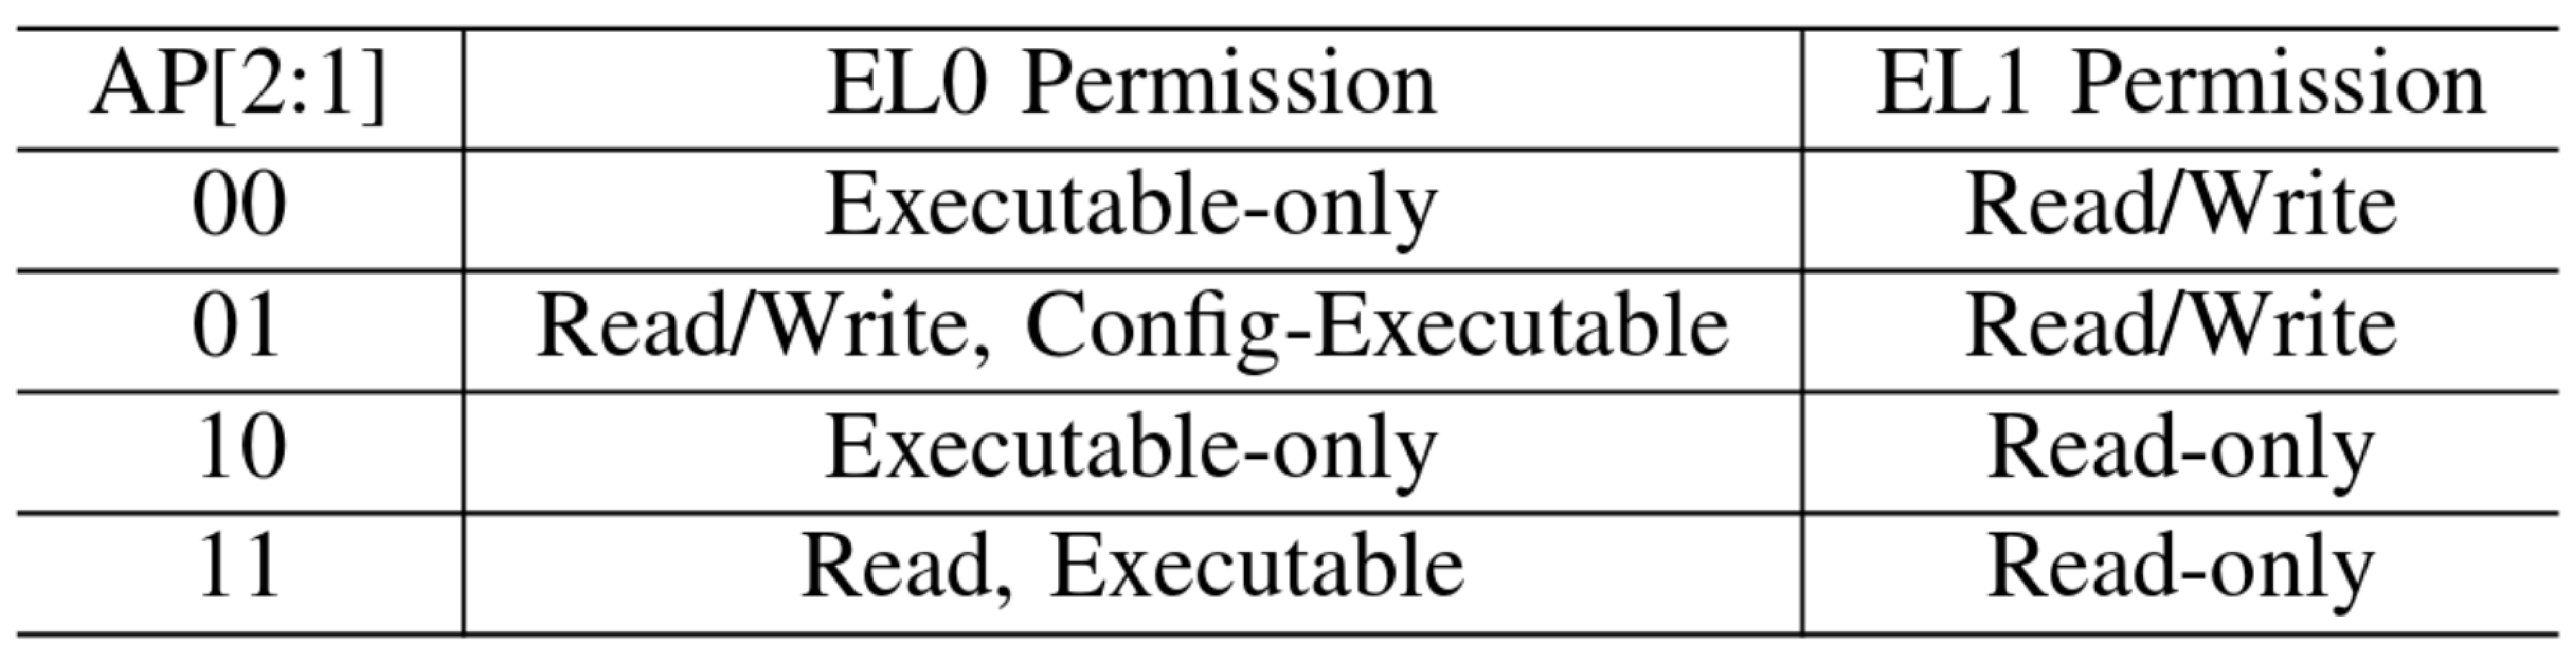
\includegraphics[width=1.0\linewidth]{figures/permission.pdf}
\end{figure}
\end{frame}

%------------------------------------------------

\section{NORAX Solution}
\begin{frame}
\frametitle{NORAX Solution}
\begin{enumerate}
\item {\large separate data and code to different pages}
\item {\large properly update all references}
\end{enumerate}
\begin{figure}
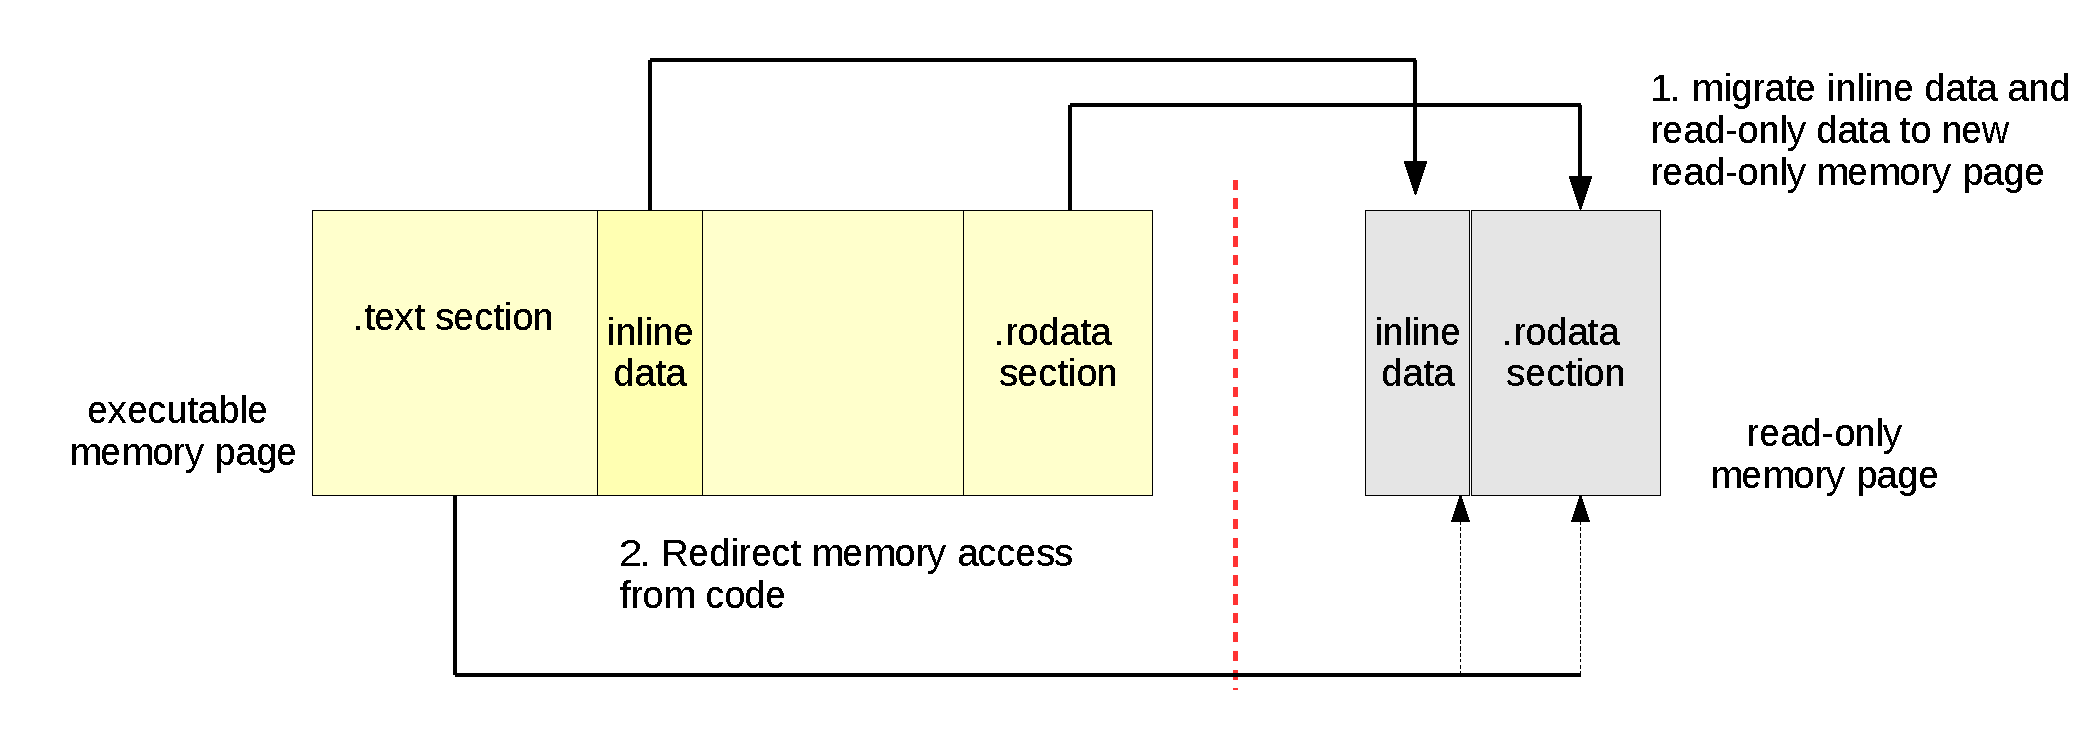
\includegraphics[width=1.0\linewidth]{figures/solution.pdf}
\end{figure}
\end{frame}

%------------------------------------------------

\section{Executable Data Relocation Sample}
\begin{frame}
\frametitle{Executable Data Relocation Sample}
\begin{figure}
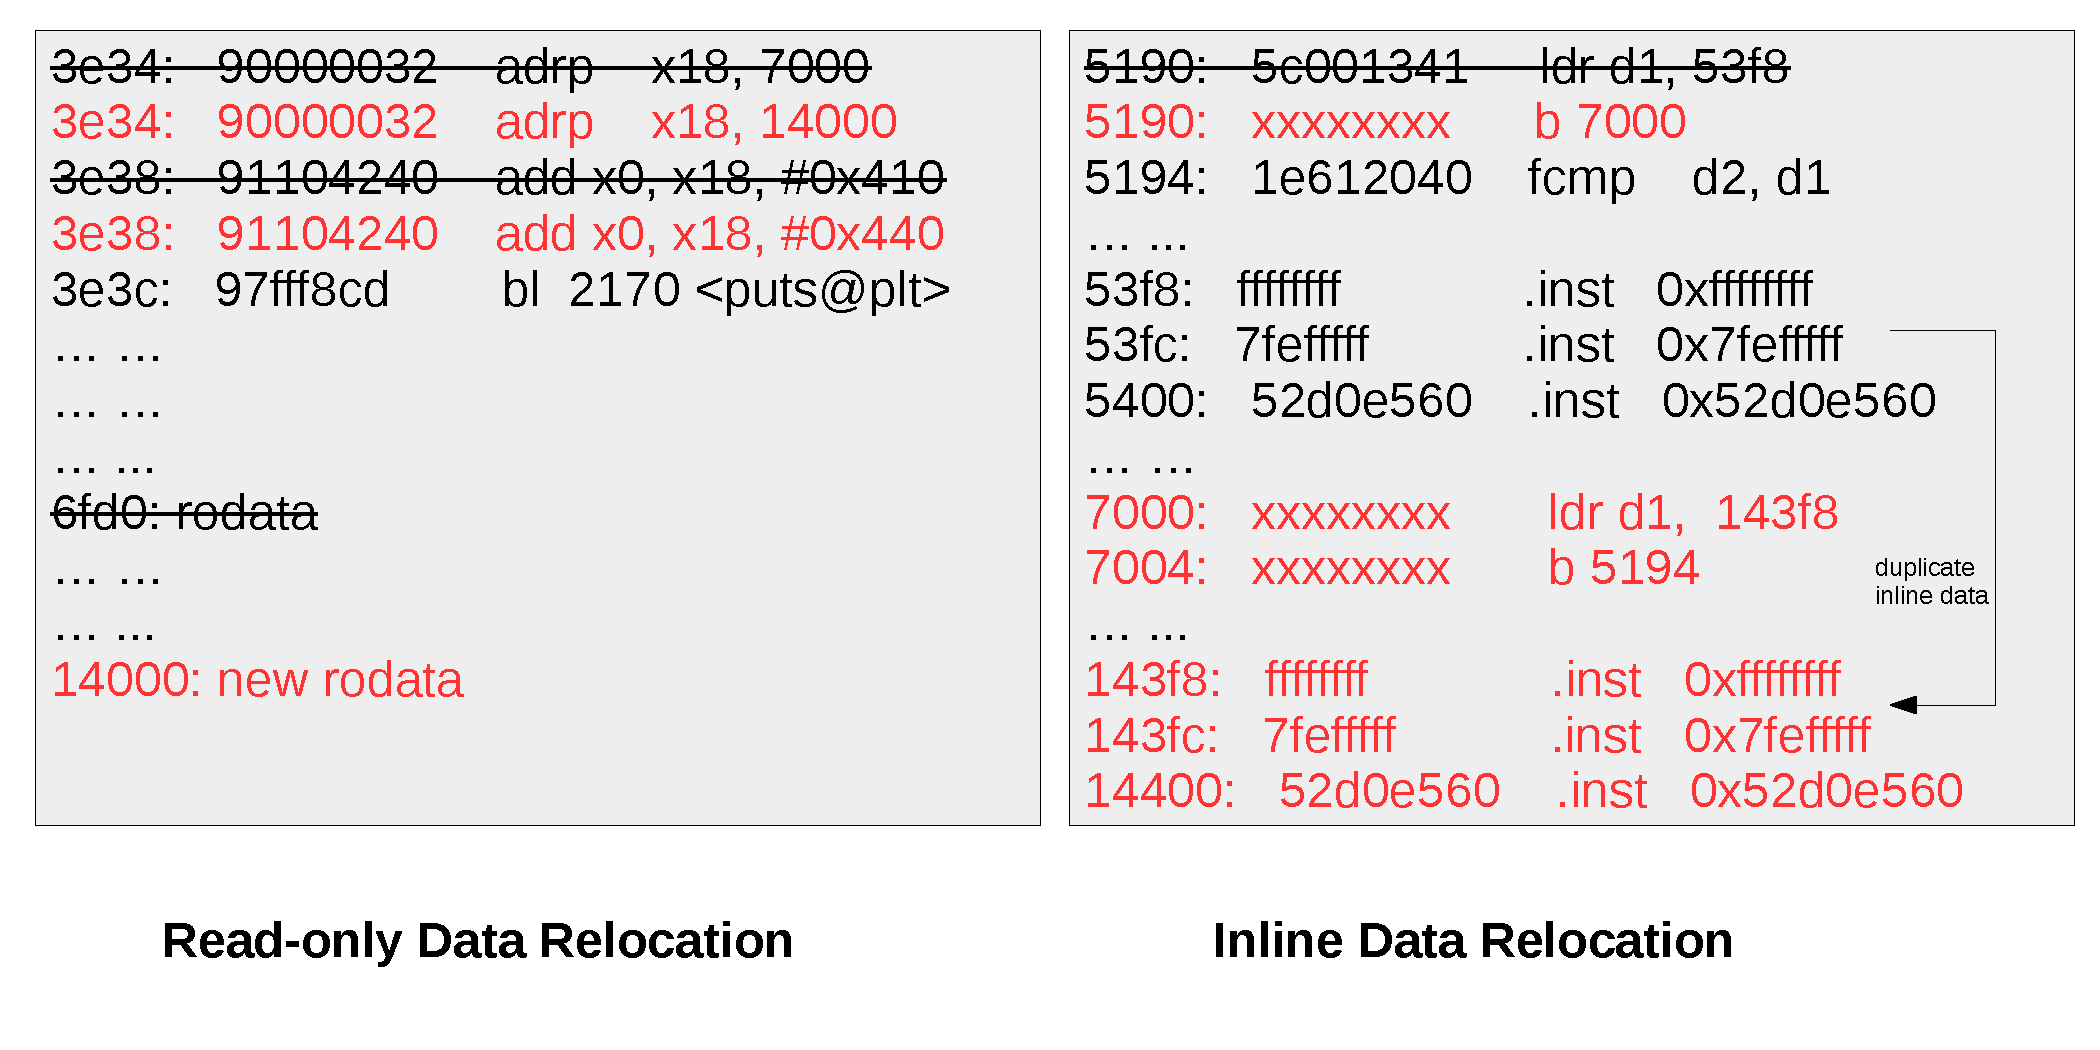
\includegraphics[width=1.0\linewidth]{figures/rodata.pdf}
\end{figure}
\end{frame}

%------------------------------------------------

\section{NORAX Challenges}
\begin{frame}
\frametitle{NORAX Challenges}
\begin{columns}[c]
\column{.70\textwidth}
\begin{itemize}
\visible<1->{\item{\large \textcolor{red}{rodata and executable inline data}}}
	\begin{itemize}
		\visible<1->{\item{\large Reference from code (.text)}}
		\visible<1->{\item{\large Reference from symbol table (.dynsym)}}
		\visible<1->{\item{\large Reference from relocation table (.rela.dyn)}}
		\visible<1->{\item{\large Reference from global offset table (.got)}}
		\visible<1->{\item{\large Reference from read-only global data (.data.rel.ro)}}
	\end{itemize}
\visible<2->{\item{\large \textcolor{red}{read-only ELF header}}}
	\begin{itemize}
		\visible<2->{\item{\large Reference from linker}}
	\end{itemize}
\visible<3->{\item{\large \textcolor{red}{.eh\_frame\_hdr/.eh\_frame}}}
	\begin{itemize}
		\visible<3->{\item{\large Reference from C++ runtime}}
	\end{itemize}
\end{itemize}
\column{.30\textwidth}
\begin{figure}

\includegraphics[width=0.7\linewidth]{figures/challenge.pdf}
\end{figure}
\end{columns}
\end{frame}

%------------------------------------------------

\section{Design Goals}
\begin{frame}
\frametitle{Design Goals}
\begin{block}{Code-Data Separation: precision vs. practical}
\begin{itemize}
\item A complete set of executable data
\item A subset of references
\end{itemize}
\end{block}
\pause
\begin{block}{Security}
\begin{itemize}
\item Expose as less code as possible
\item Enforce policy based security on missed references
\end{itemize}
\end{block}
\pause
\begin{block}{Practicability}
\begin{itemize}
\item Low runtime and memory overhead
\item Non-exclusive binary hardening solution
\item Backward compatibility
\item Modularity support
\end{itemize}
\end{block}
\end{frame}

%------------------------------------------------

\section{NORAX Framework}
\begin{frame}
\frametitle{NORAX Framework}
\begin{itemize}
\item NDisassembler: collect executable data and references
\item NPatcher: static binary transformation
\item NLoader: update executable data references
\item NMonitor: runtime policy check for false-positive
\end{itemize}
\begin{figure}
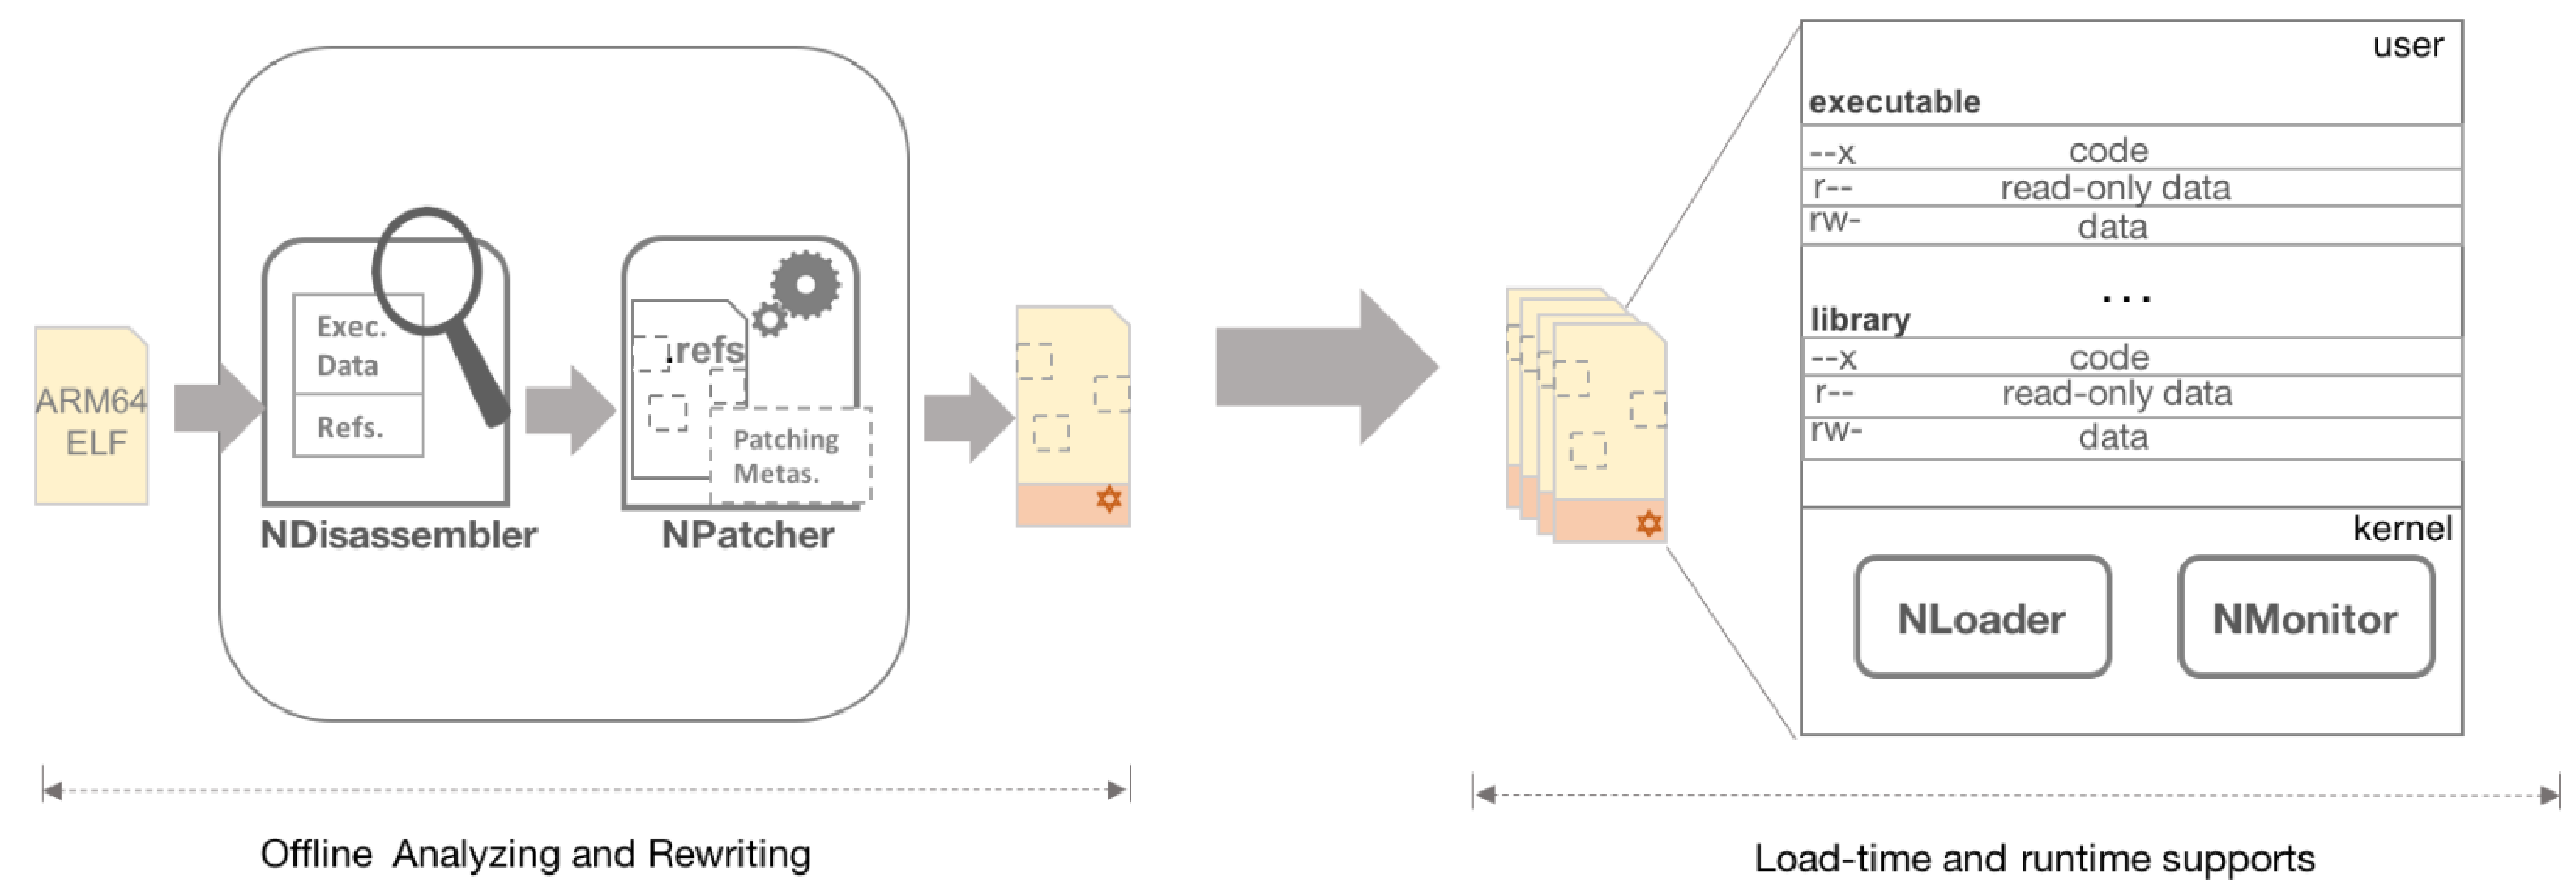
\includegraphics[width=1.0\linewidth]{figures/framework.pdf}
\end{figure}
\end{frame}

%------------------------------------------------

\section{NORAX: NDisassembler}
\begin{frame}
\frametitle{NORAX: NDisassembler}
\begin{columns}[c]
\column{.65\textwidth}
\begin{itemize}
\item \textit{Algorithm 1} and \textit{Algorithm 2} in NORAX paper for details
\begin{enumerate}
\item Linear-sweep disassembly (objdump -d)
\item Identify executable data position (rodata or inline) and reference (adr(p) or ldr)
\item For unbounded data, collect a set of over-approximated date via Unbounded Data Expansion (Algorithm 2)
\end{enumerate}
\end{itemize}
\column{.35\textwidth}
\begin{figure}
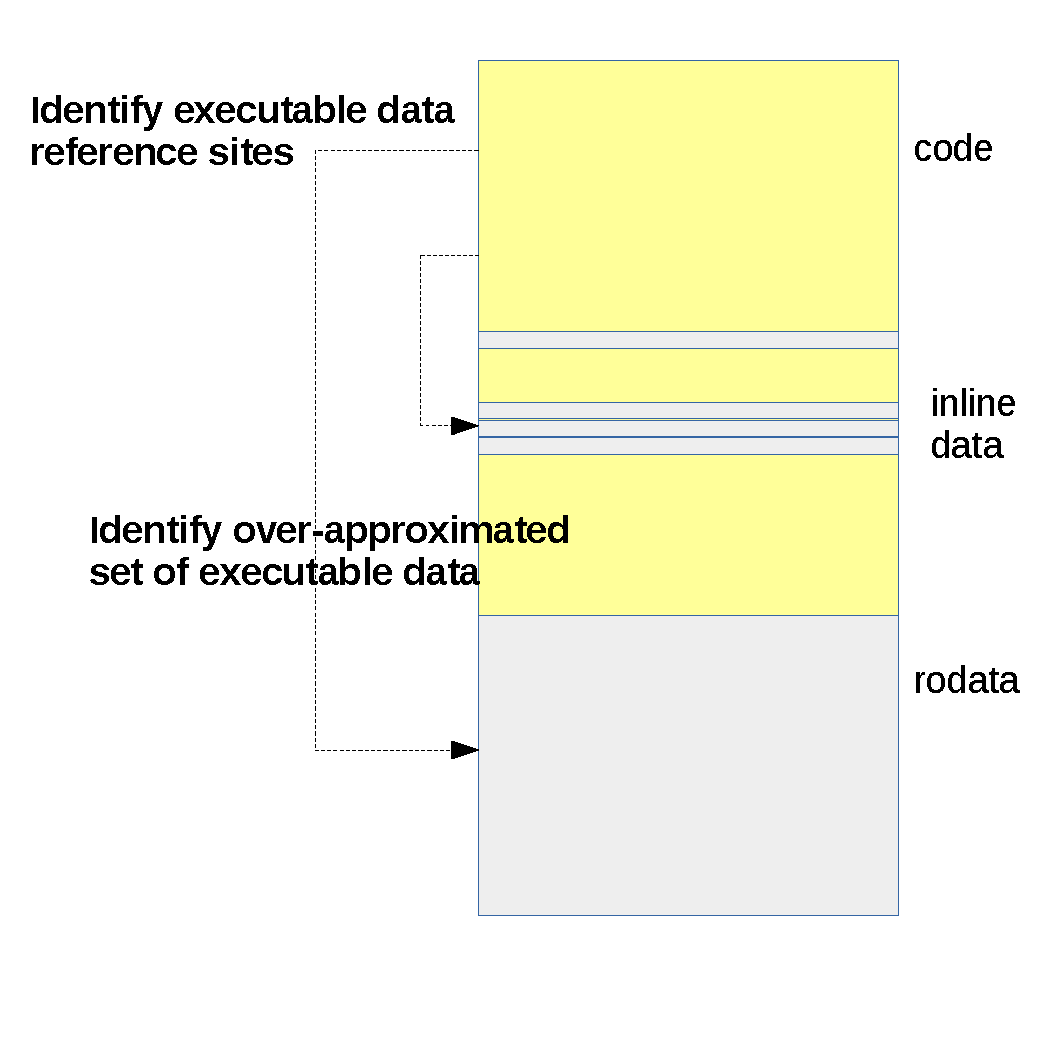
\includegraphics[width=1.0\linewidth]{figures/ndisassembler.pdf}
\end{figure}
\end{columns}
\end{frame}

%------------------------------------------------

\section{NORAX: NPatcher}
\begin{frame}
\frametitle{NORAX: NPatcher}
\begin{columns}[c]
\column{.65\textwidth}
\begin{itemize}
\item New memory layout
	\begin{itemize}
		\item New location of the executable data
		\item Take into consideration reference addressing range, and emit stub code if needed
	\end{itemize}
\item Append NORAX-related metadata to the end
	\begin{itemize}
		\item Duplicated inline data
		\item References locations and displacements
		\item Stub code
		\item NORAX header
	\end{itemize}
\end{itemize}
\column{.35\textwidth}
\begin{figure}
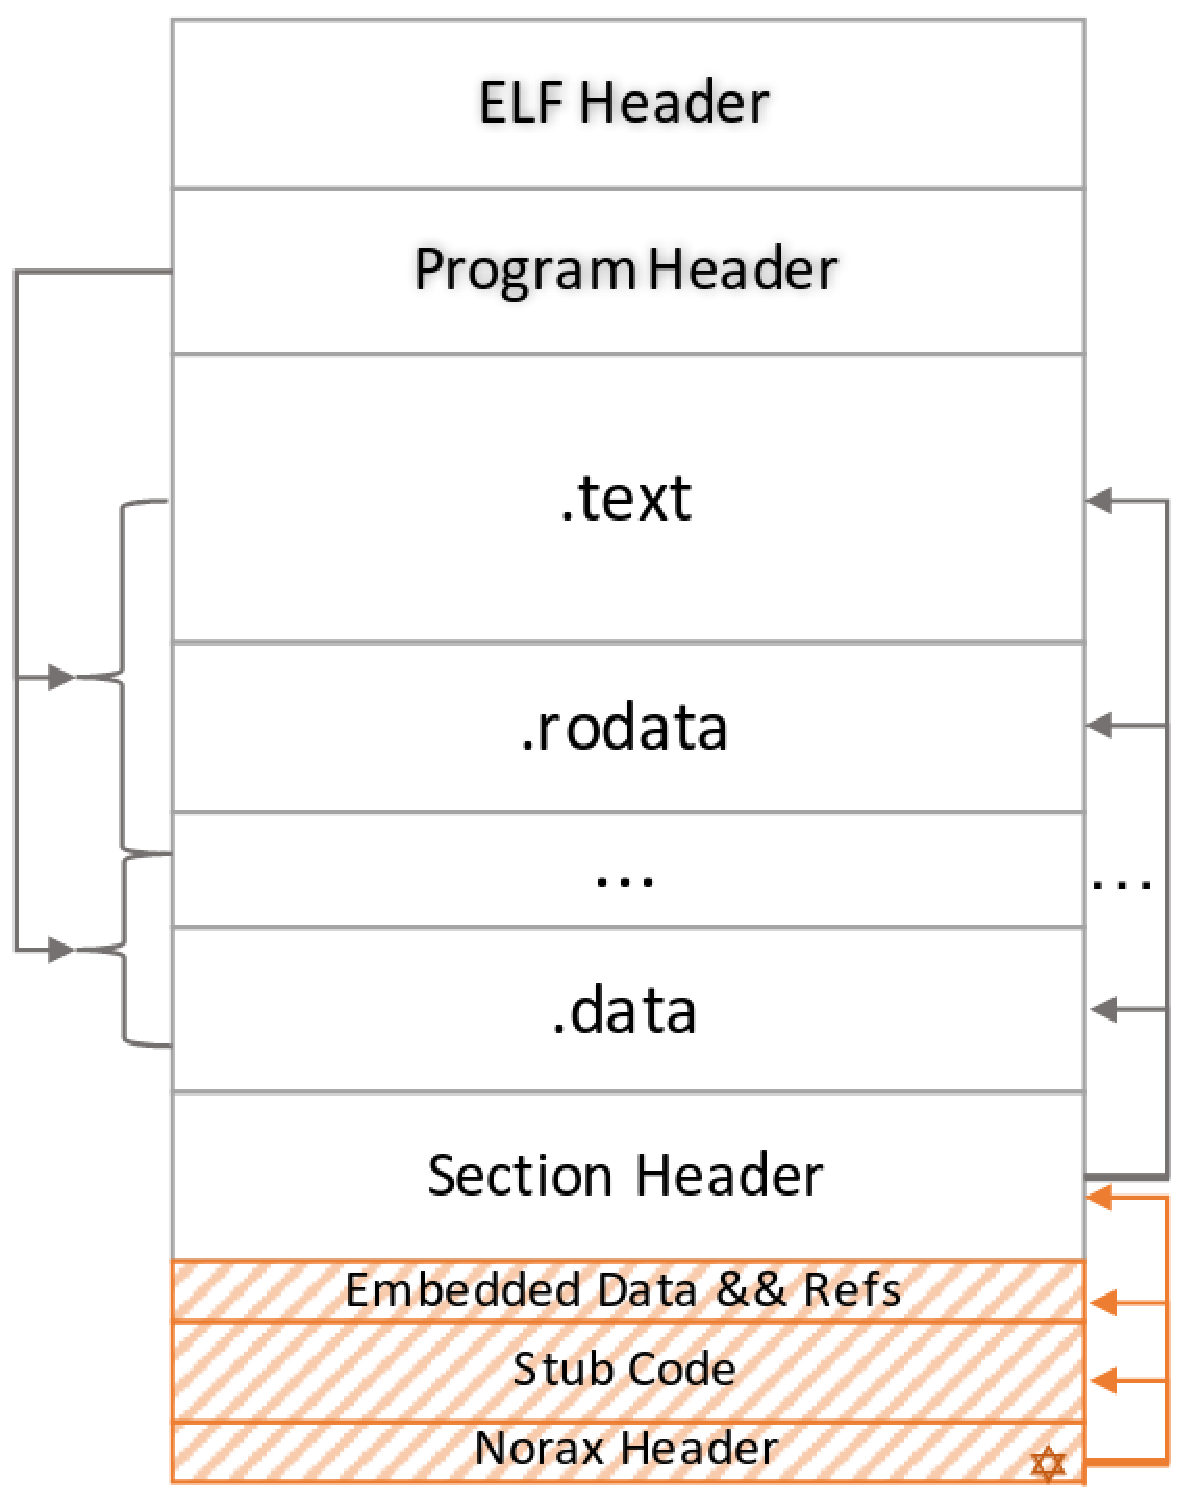
\includegraphics[width=1.0\linewidth]{figures/npatcher.pdf}
\end{figure}
\end{columns}
\end{frame}

%------------------------------------------------

\section{NORAX: NLoader}
\begin{frame}
\frametitle{NORAX: NLoader}
\begin{columns}[c]
\column{.50\textwidth}
\begin{itemize}
\item \textbf{Ld-1: }Setup NORAX book-keeping data and new mapping of read-only data and sections
\item \textbf{Ld-2: }Redirect .dynamic access to new read-only sections
\item \textbf{Ld-3: }Adjust all referencees and enable XOM
\end{itemize}
\column{.50\textwidth}
\begin{figure}
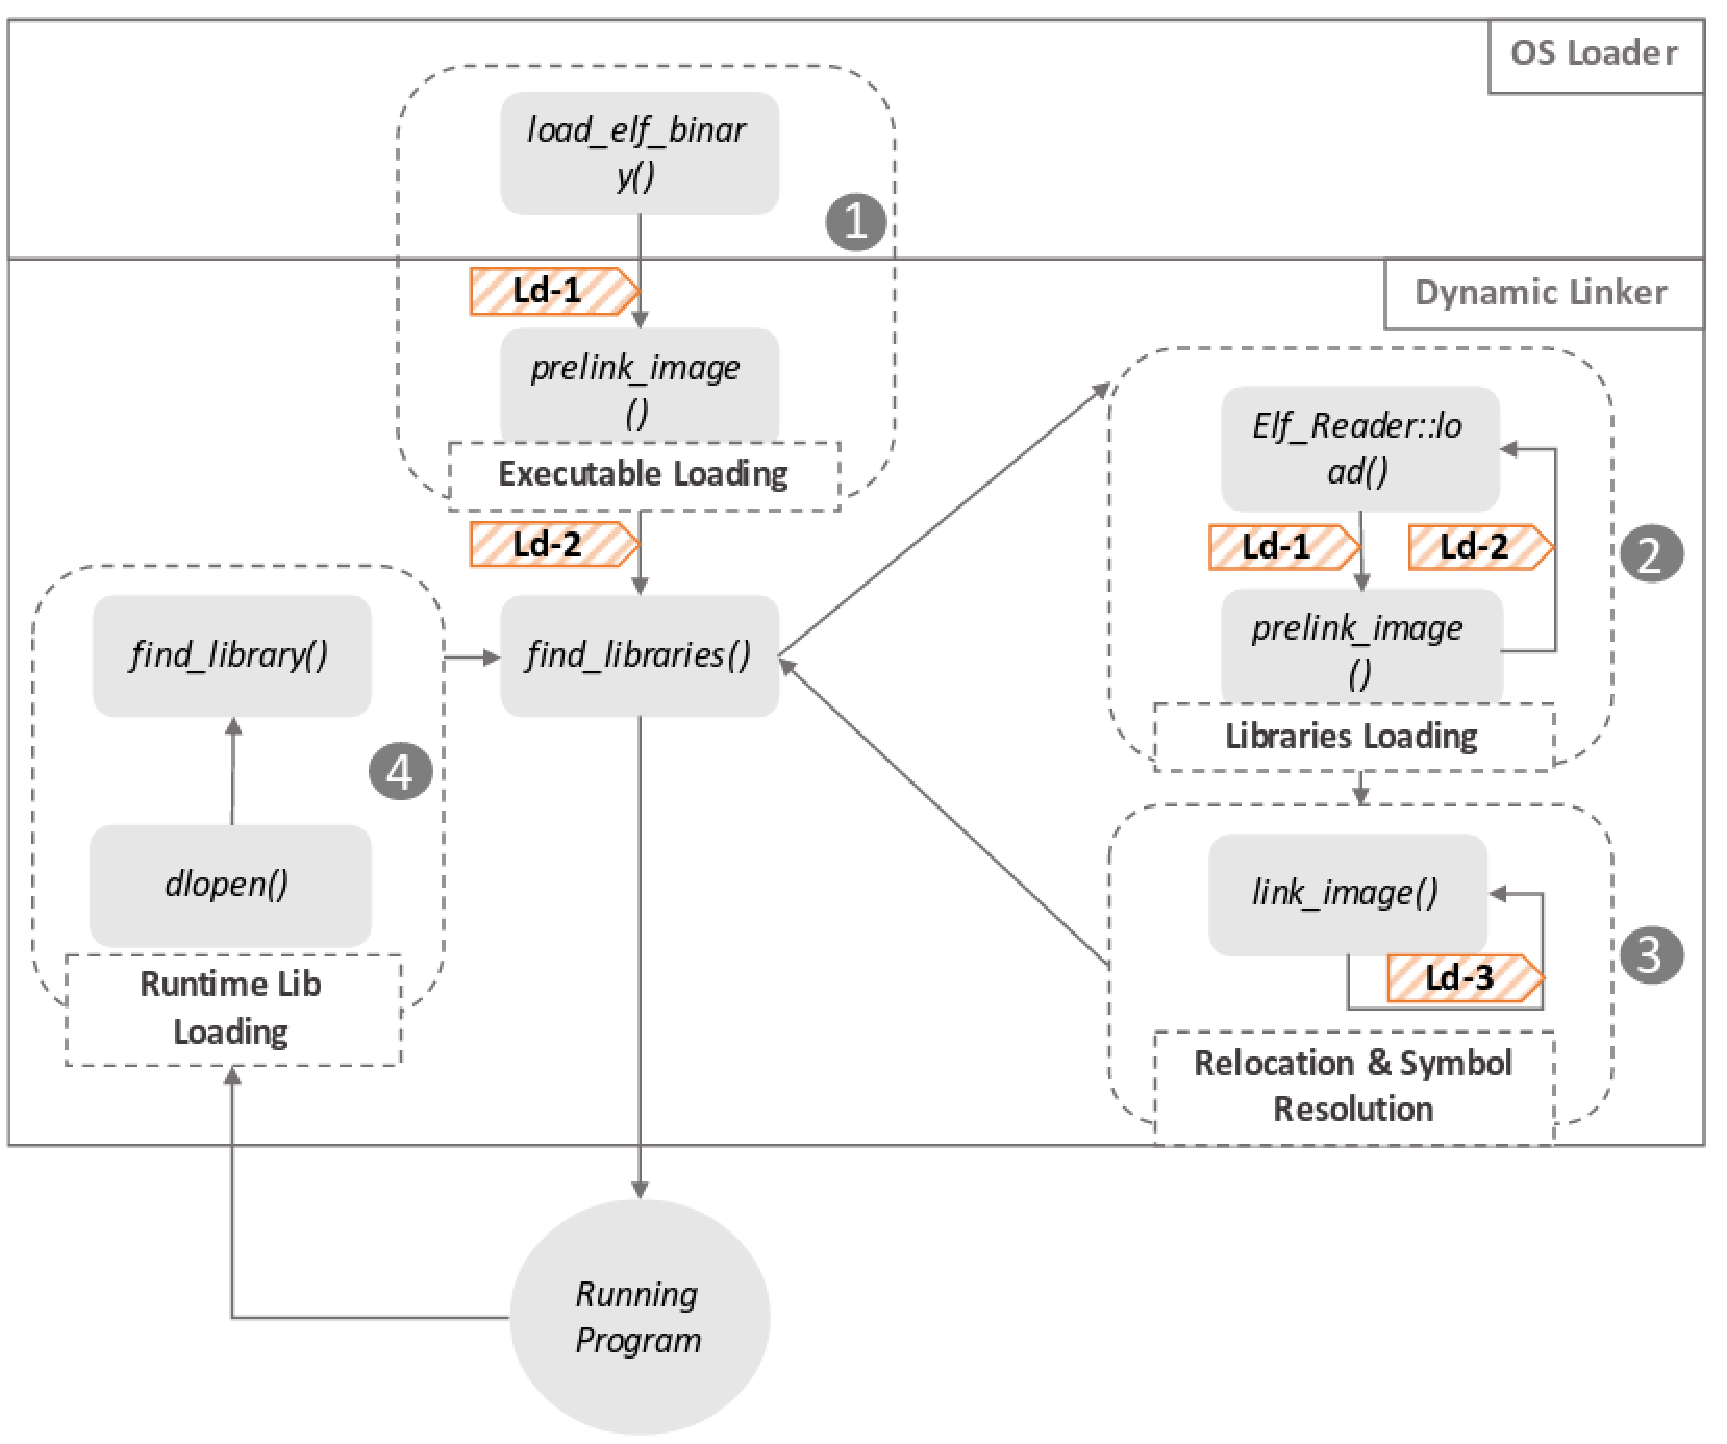
\includegraphics[width=1.0\linewidth]{figures/nloader.pdf}
\end{figure}
\end{columns}
\end{frame}

%------------------------------------------------

\section{NORAX: NMonitor}
\begin{frame}
\frametitle{NORAX: NMonitor}
\begin{columns}[c]
\column{.60\textwidth}
\begin{itemize}
\item Missed reference to embedded data
	\begin{itemize}
		\item NDisassembler may miss some references
	\end{itemize}
\item Reference to .eh\_frame\_hdr and .eh\_frame
\end{itemize}
\column{.40\textwidth}
\begin{figure}
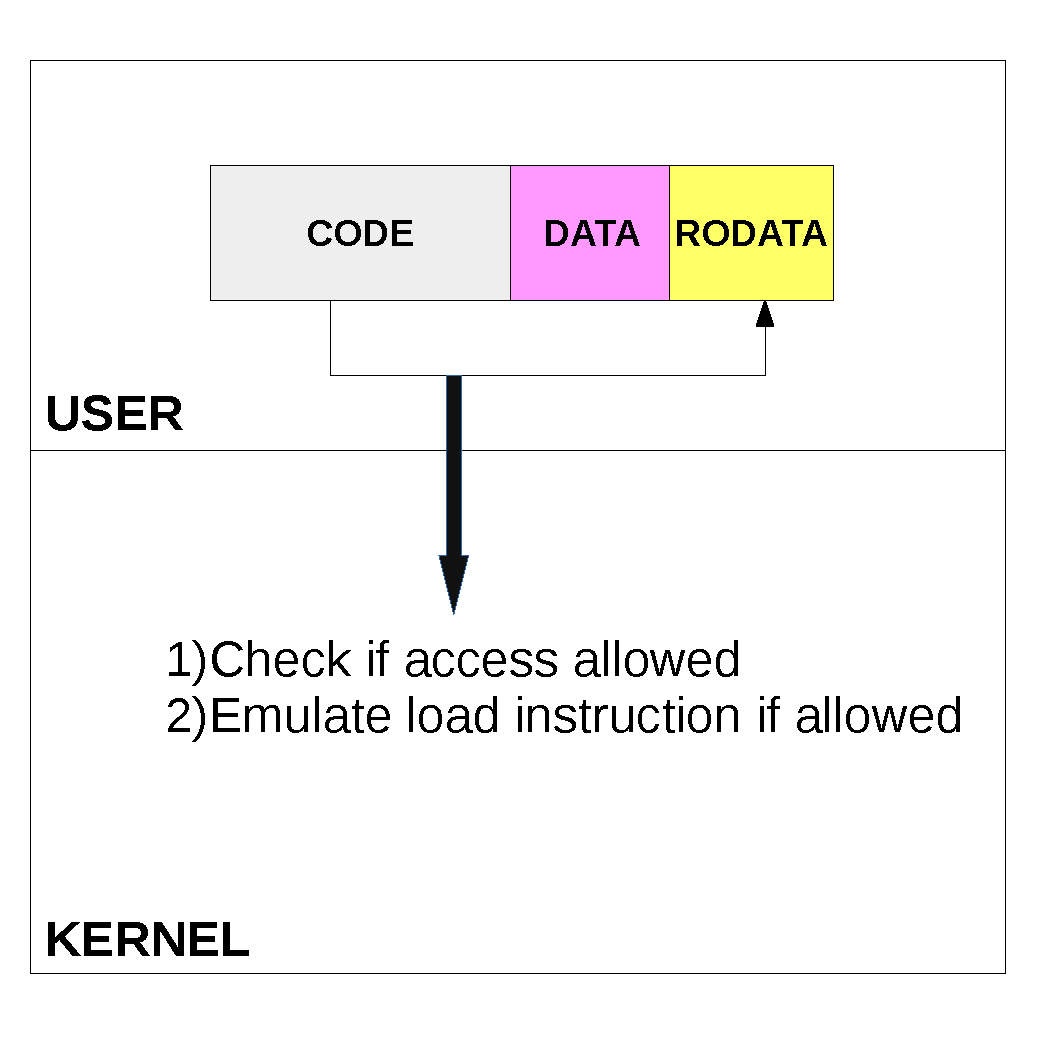
\includegraphics[width=1.0\linewidth]{figures/nmonitor.pdf}
\end{figure}
\end{columns}
\end{frame}

%------------------------------------------------

\section{Evaluation - transformation correctness}
\begin{frame}
\frametitle{Evaluation - transformation correctness}
\begin{columns}[c]
\column{.5\textwidth}
\begin{itemize}
%\setlength\itemsep{1em}
\item LG Nexus 5X (Qualcomm Snapdragon 808MSM8992 (4 x ARM Cortex-A53 \& 2 x ARM Cortex-A57), and 2GB RAM)
\item Android OS v6.0.1 (Marshmallow) with Linux kernel v3.14 (64-bit)
\item Changed bionic linker and linux kernel
\item Tested for 20 core system binaries
\end{itemize}
\begin{center}
\begin{figure}
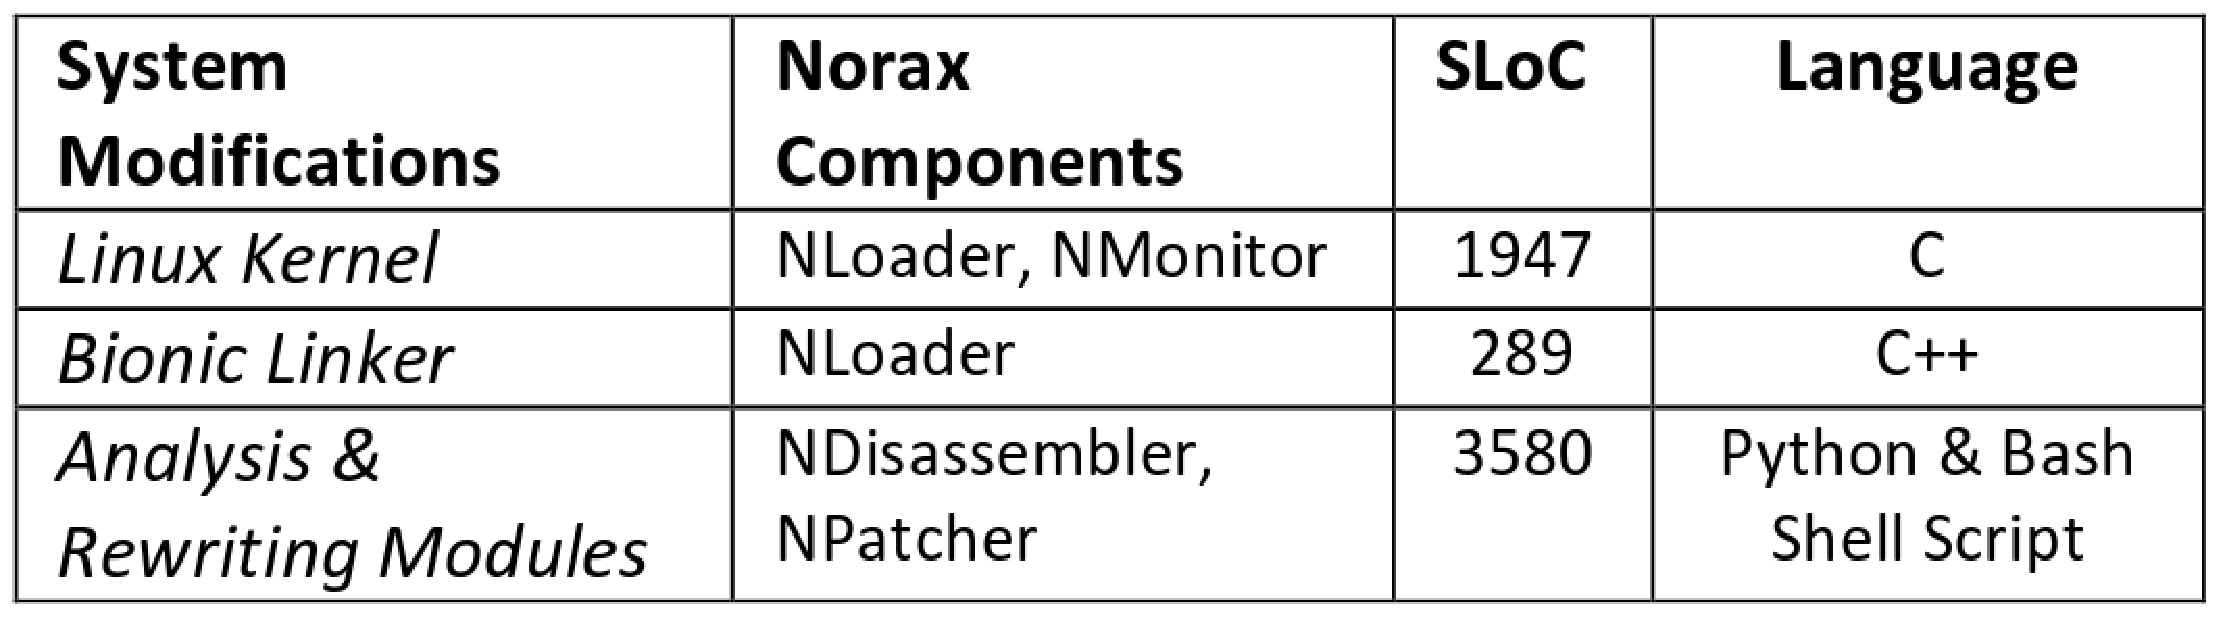
\includegraphics[width=.8\linewidth]{figures/loc.pdf}
\end{figure}
\end{center}
\column{.5\textwidth}
\begin{center}
\begin{figure}
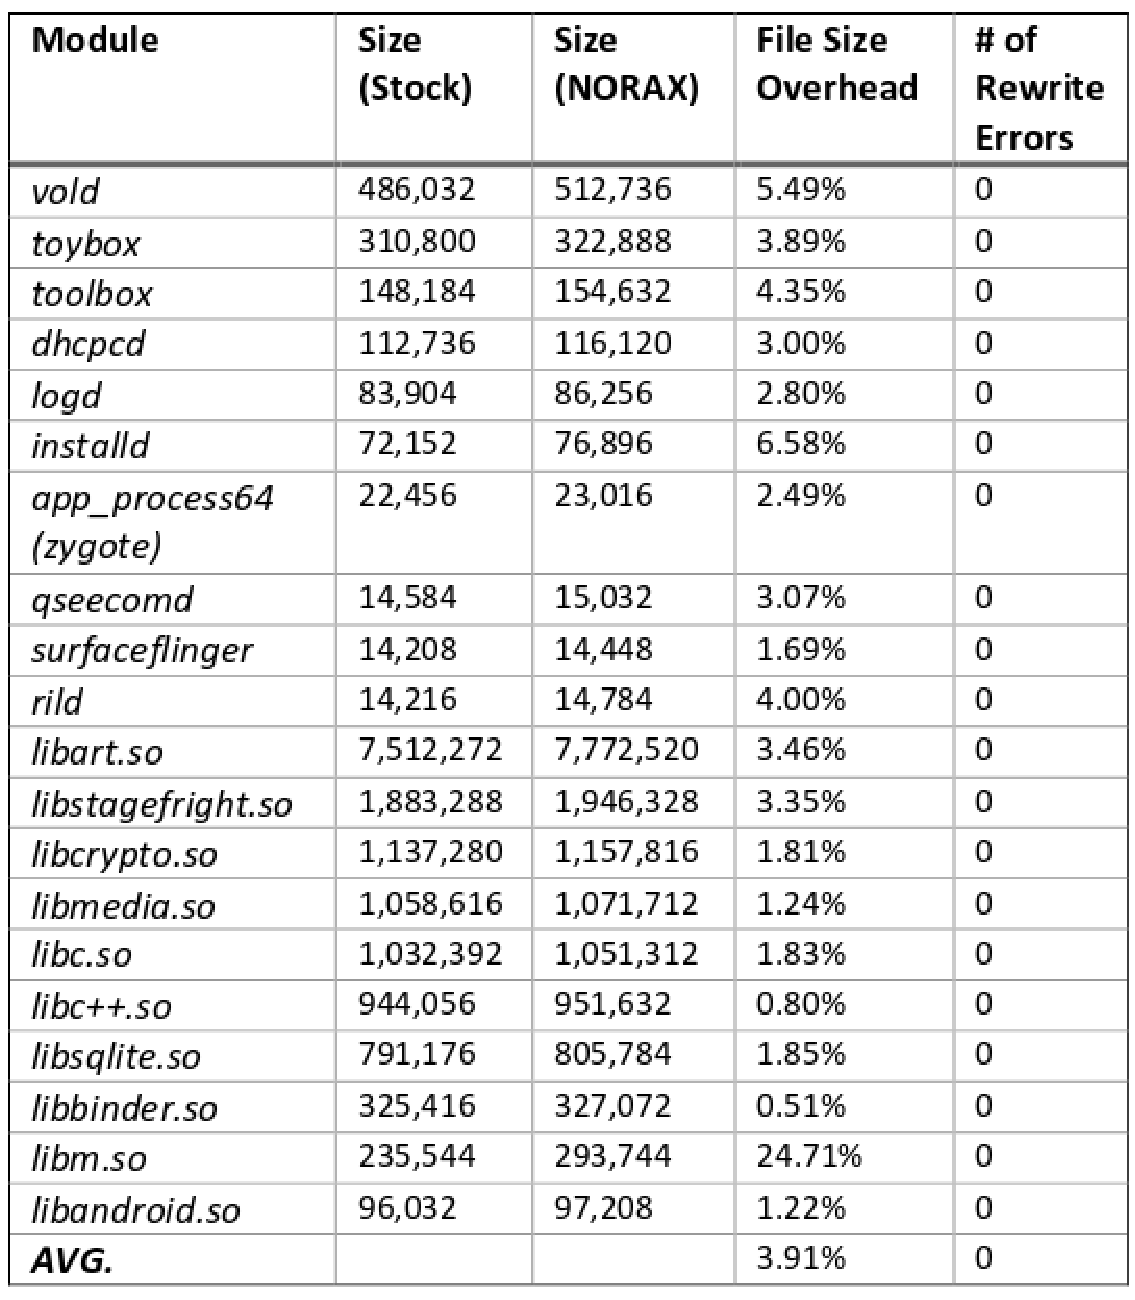
\includegraphics[width=.8\linewidth]{figures/eval-correct.pdf}
\end{figure}
\end{center}
\end{columns}
\end{frame}

%------------------------------------------------

\section{Evaluation - functionality test}
\begin{frame}
\frametitle{Evaluation - functionality test}
\begin{columns}[c]
\column{.50\textwidth}
\begin{figure}
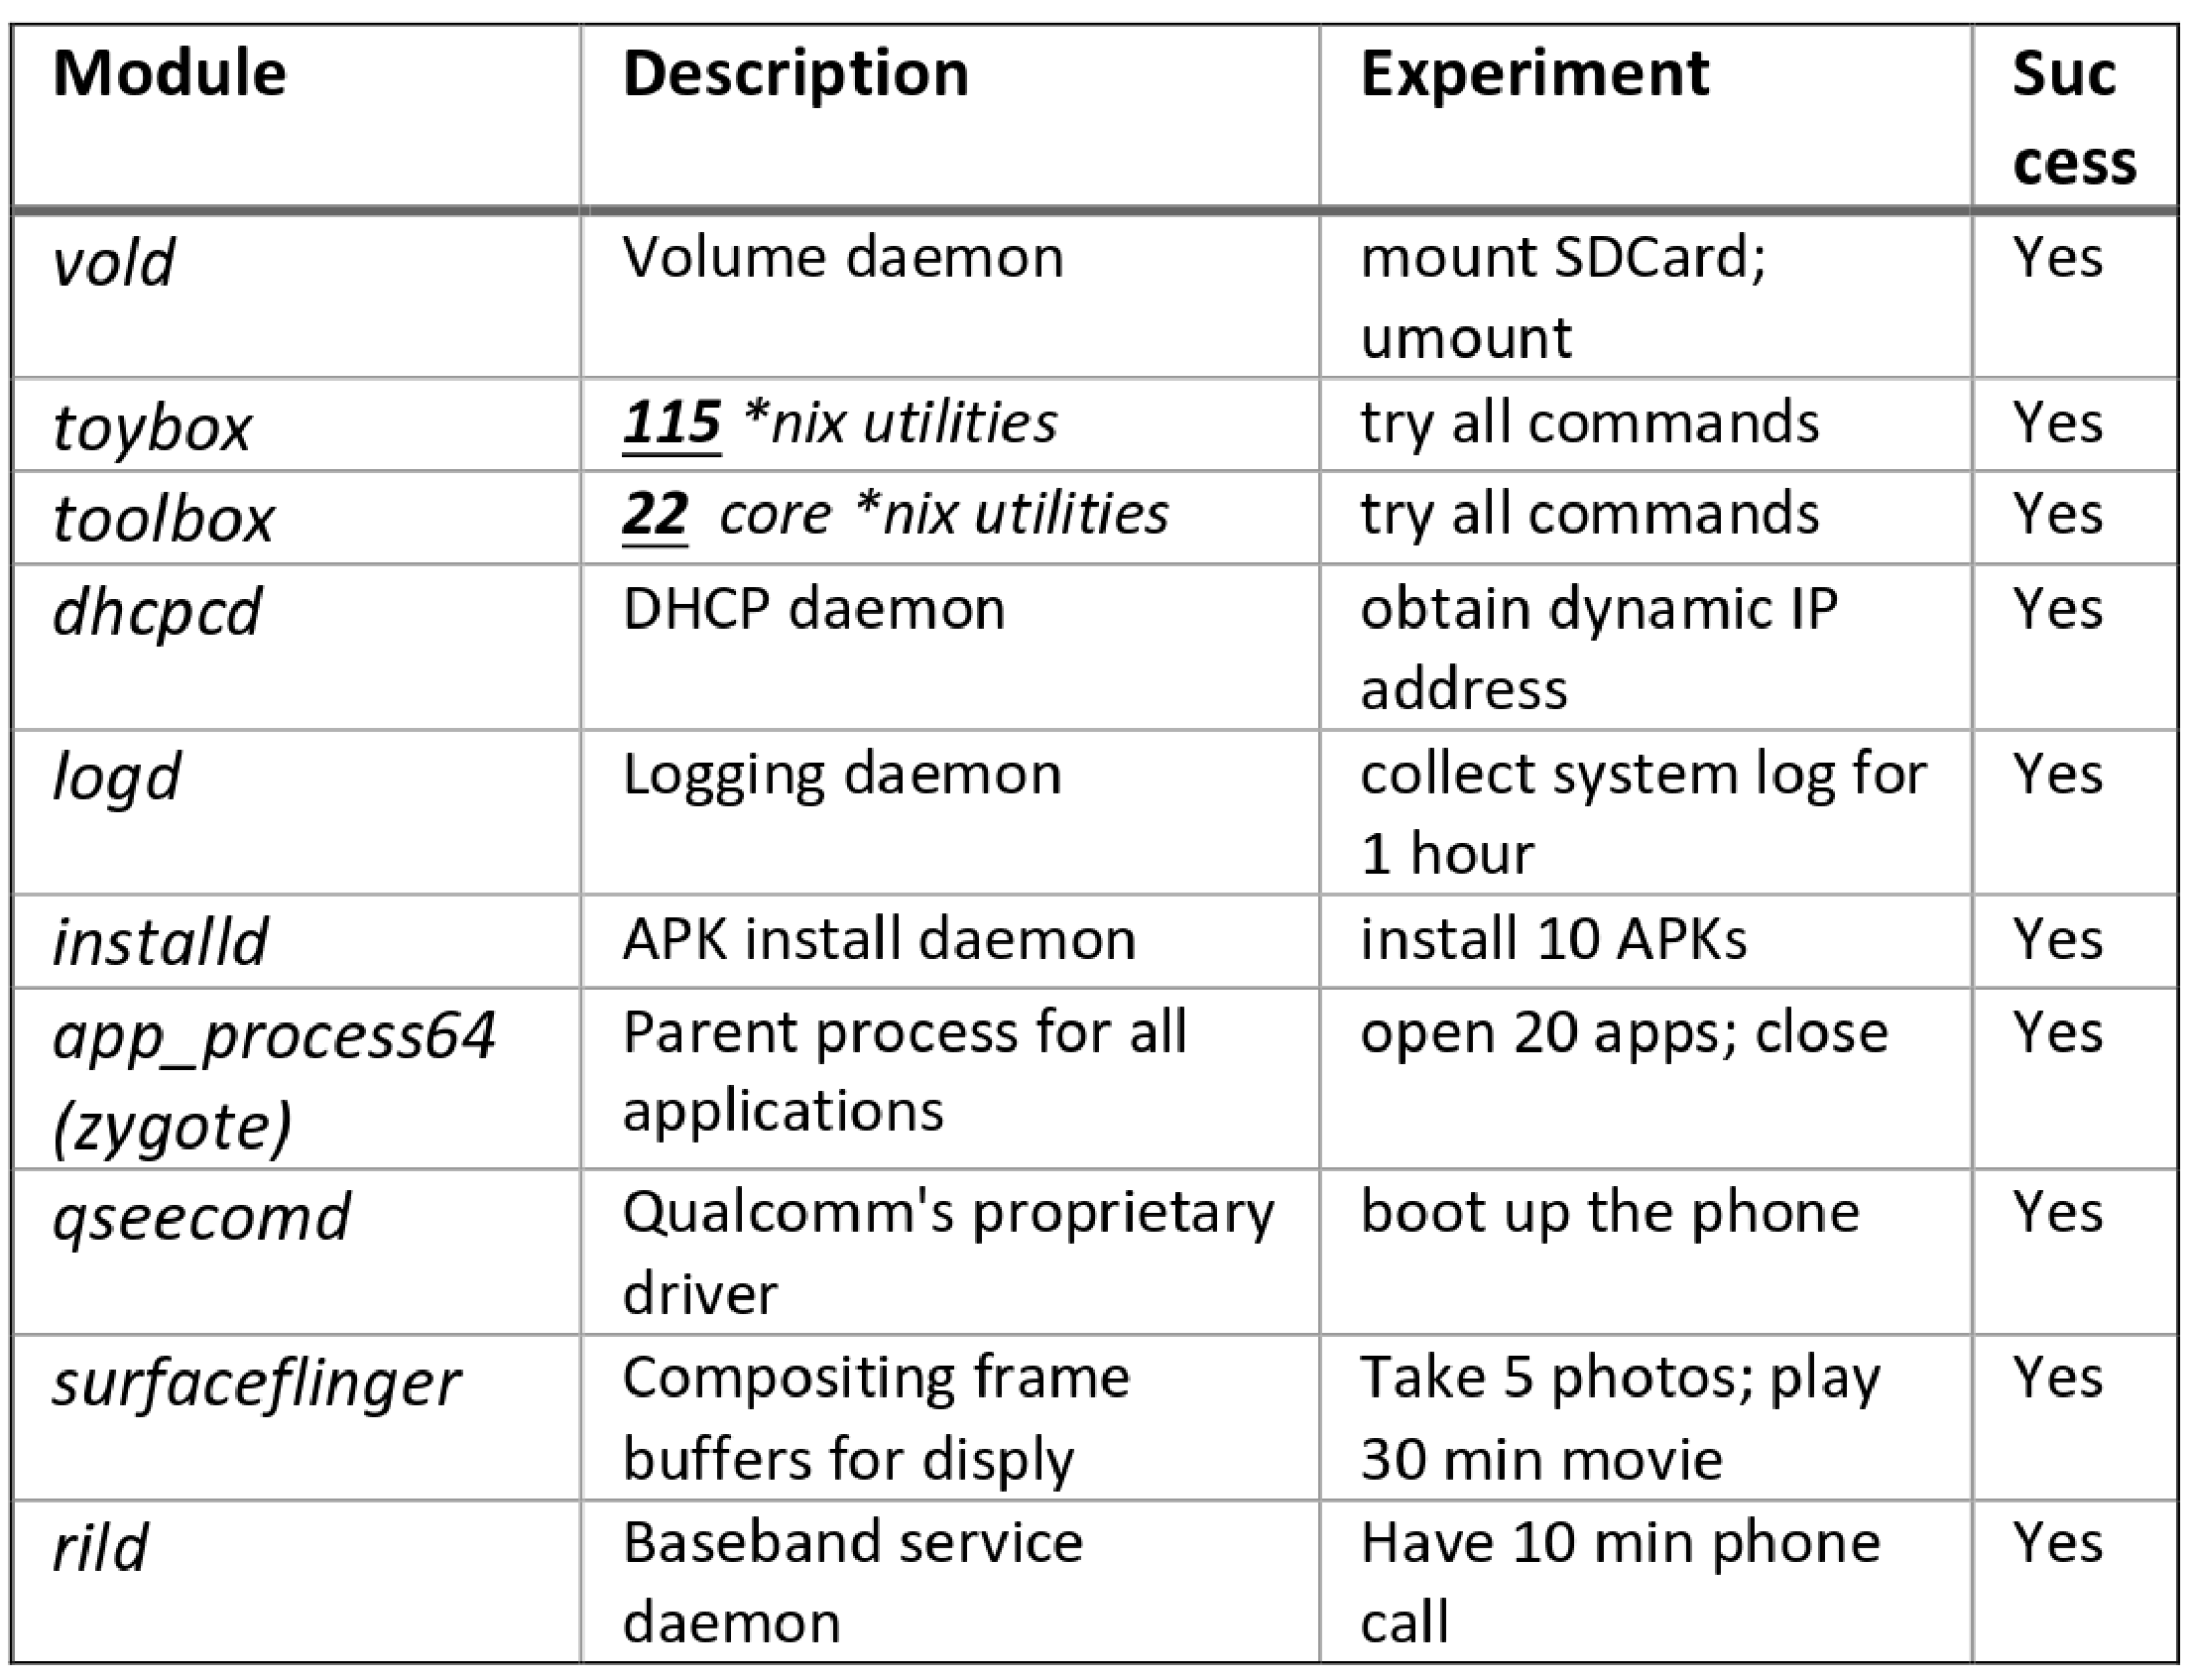
\includegraphics[width=1.0\linewidth]{figures/eval-function.pdf}
\caption{Functionality Test Result}
\end{figure}
\column{.50\textwidth}
\begin{figure}
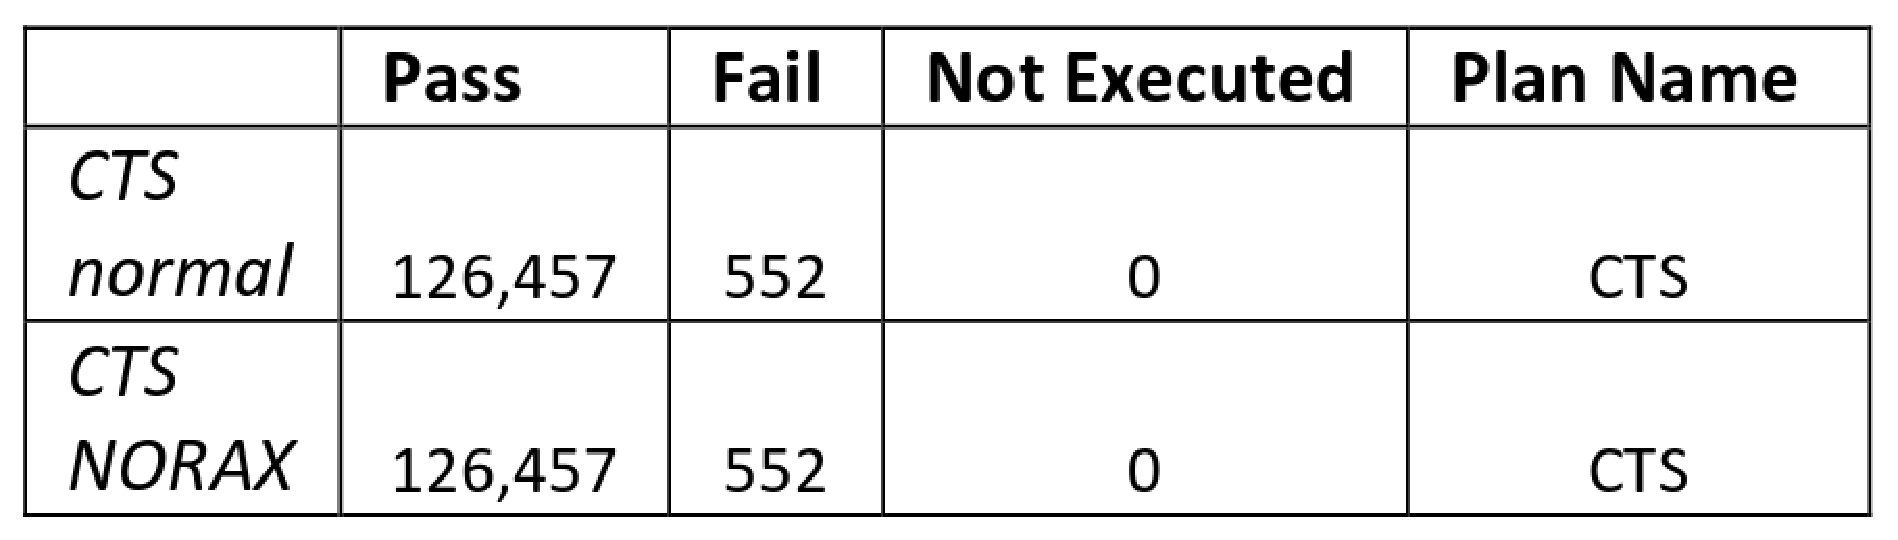
\includegraphics[width=1.0\linewidth]{figures/eval-compatibility.pdf}
\caption{Compatibility evaluation with Android Compatibility Test Suite (CTS)}
\end{figure}
\end{columns}
\end{frame}

%------------------------------------------------

\section{Evaluation - embedded data identification}
\begin{frame}
\frametitle{Evaluation - embedded data identification}
\begin{columns}[c]
\column{.50\textwidth}
\begin{itemize}
\item ground truth: compiled with debugging sections (dwarf .debug\_*)
\item very few gadgets in extracted inline data
\end{itemize}
\column{.50\textwidth}
\begin{figure}
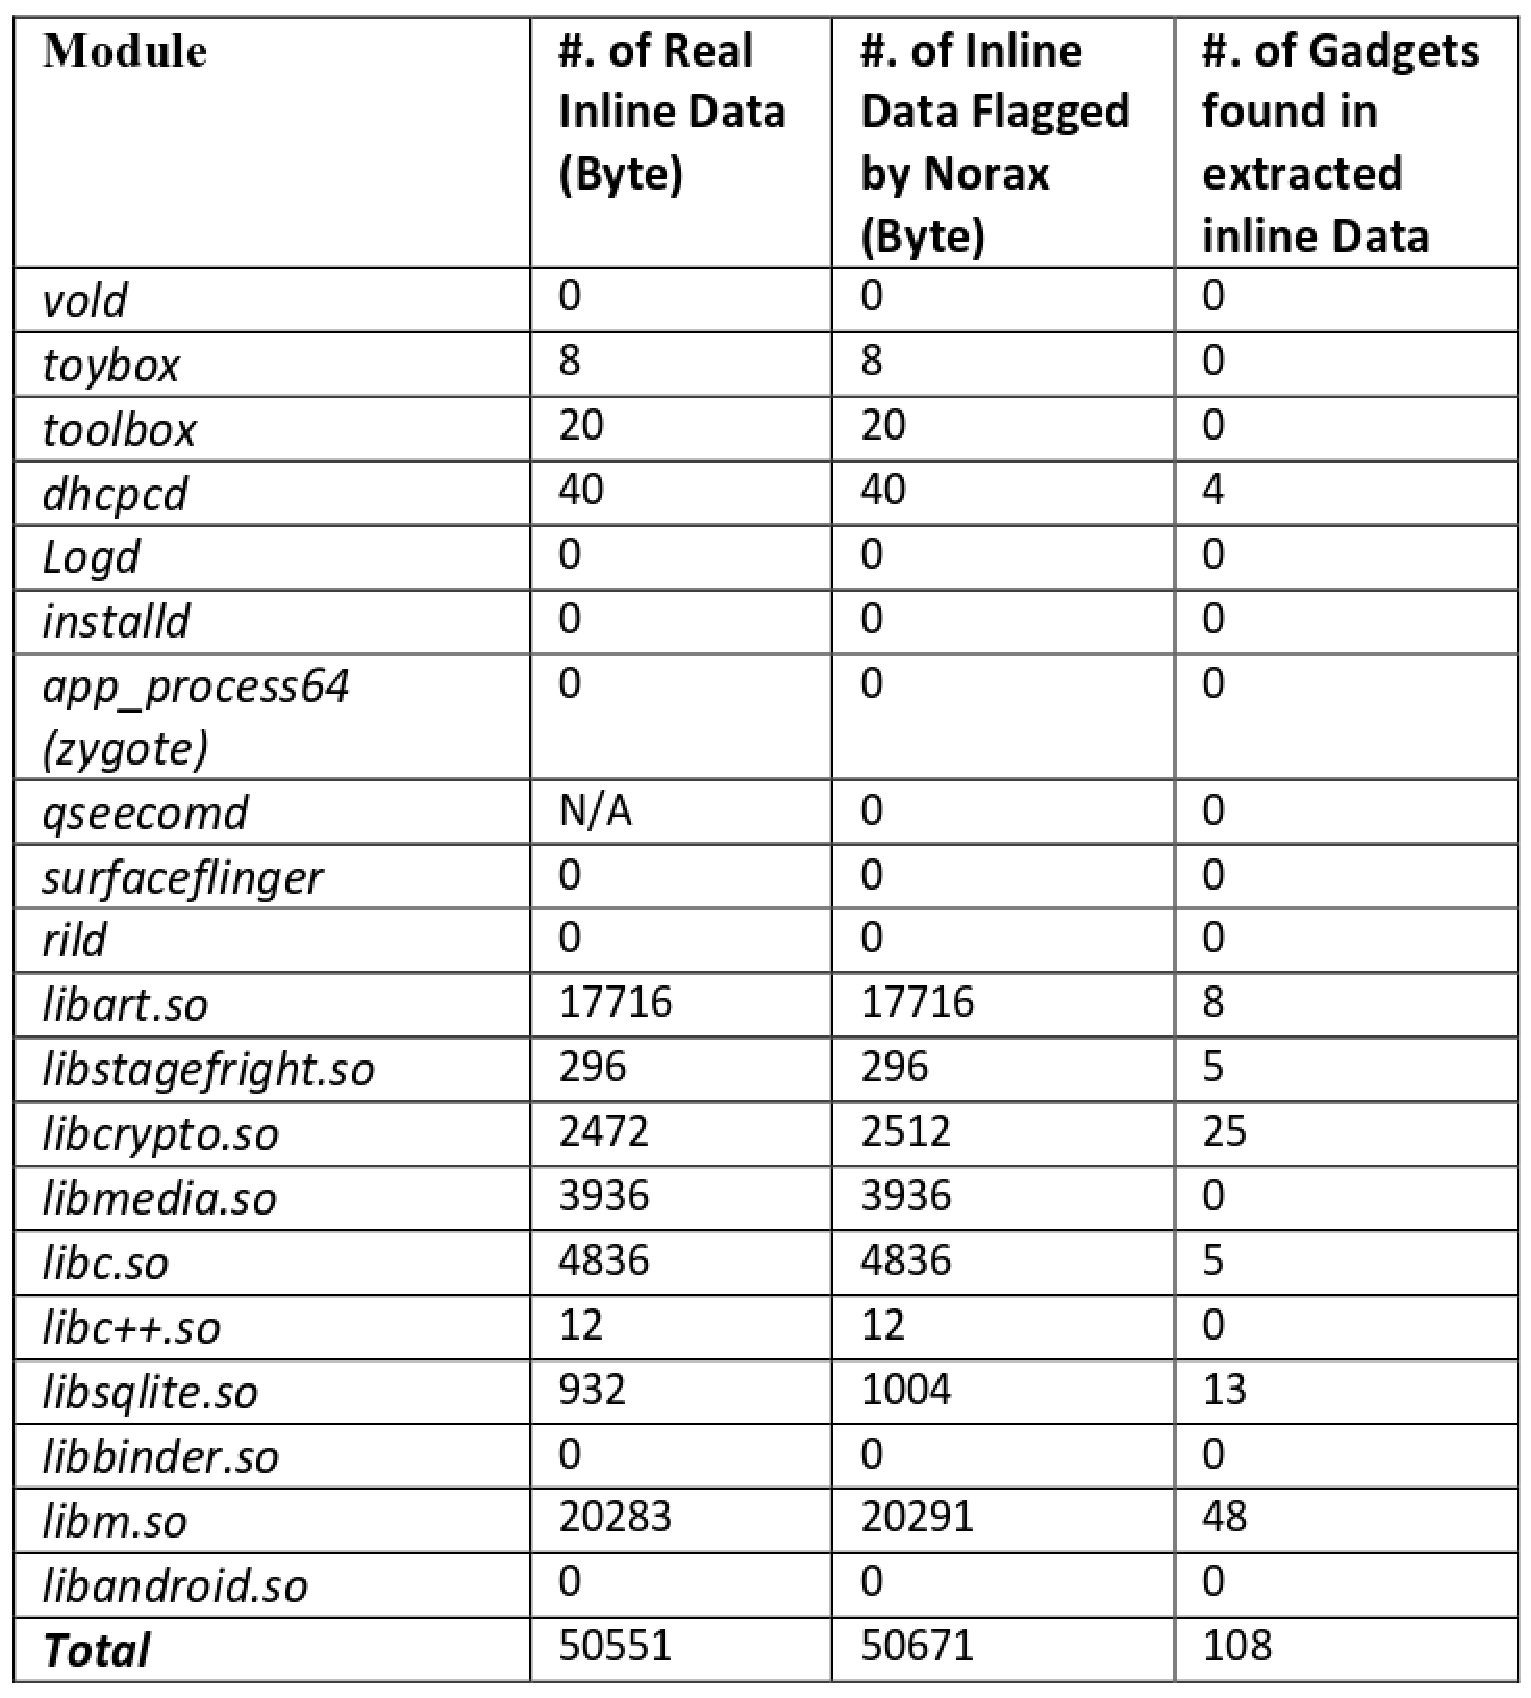
\includegraphics[width=0.8\linewidth]{figures/eval-identification.pdf}
\end{figure}
\end{columns}
\end{frame}

%------------------------------------------------

\section{Evaluation - performance}
\begin{frame}
\frametitle{Evaluation - performance}
\begin{columns}[c]
\column{.30\textwidth}
\begin{itemize}
\item average performance overhead: \textbf{\textcolor{red}{1.18\%}}
\item average memory overhead: \textbf{\textcolor{red}{2.21\%}}
\end{itemize}
\column{.70\textwidth}
\begin{figure}
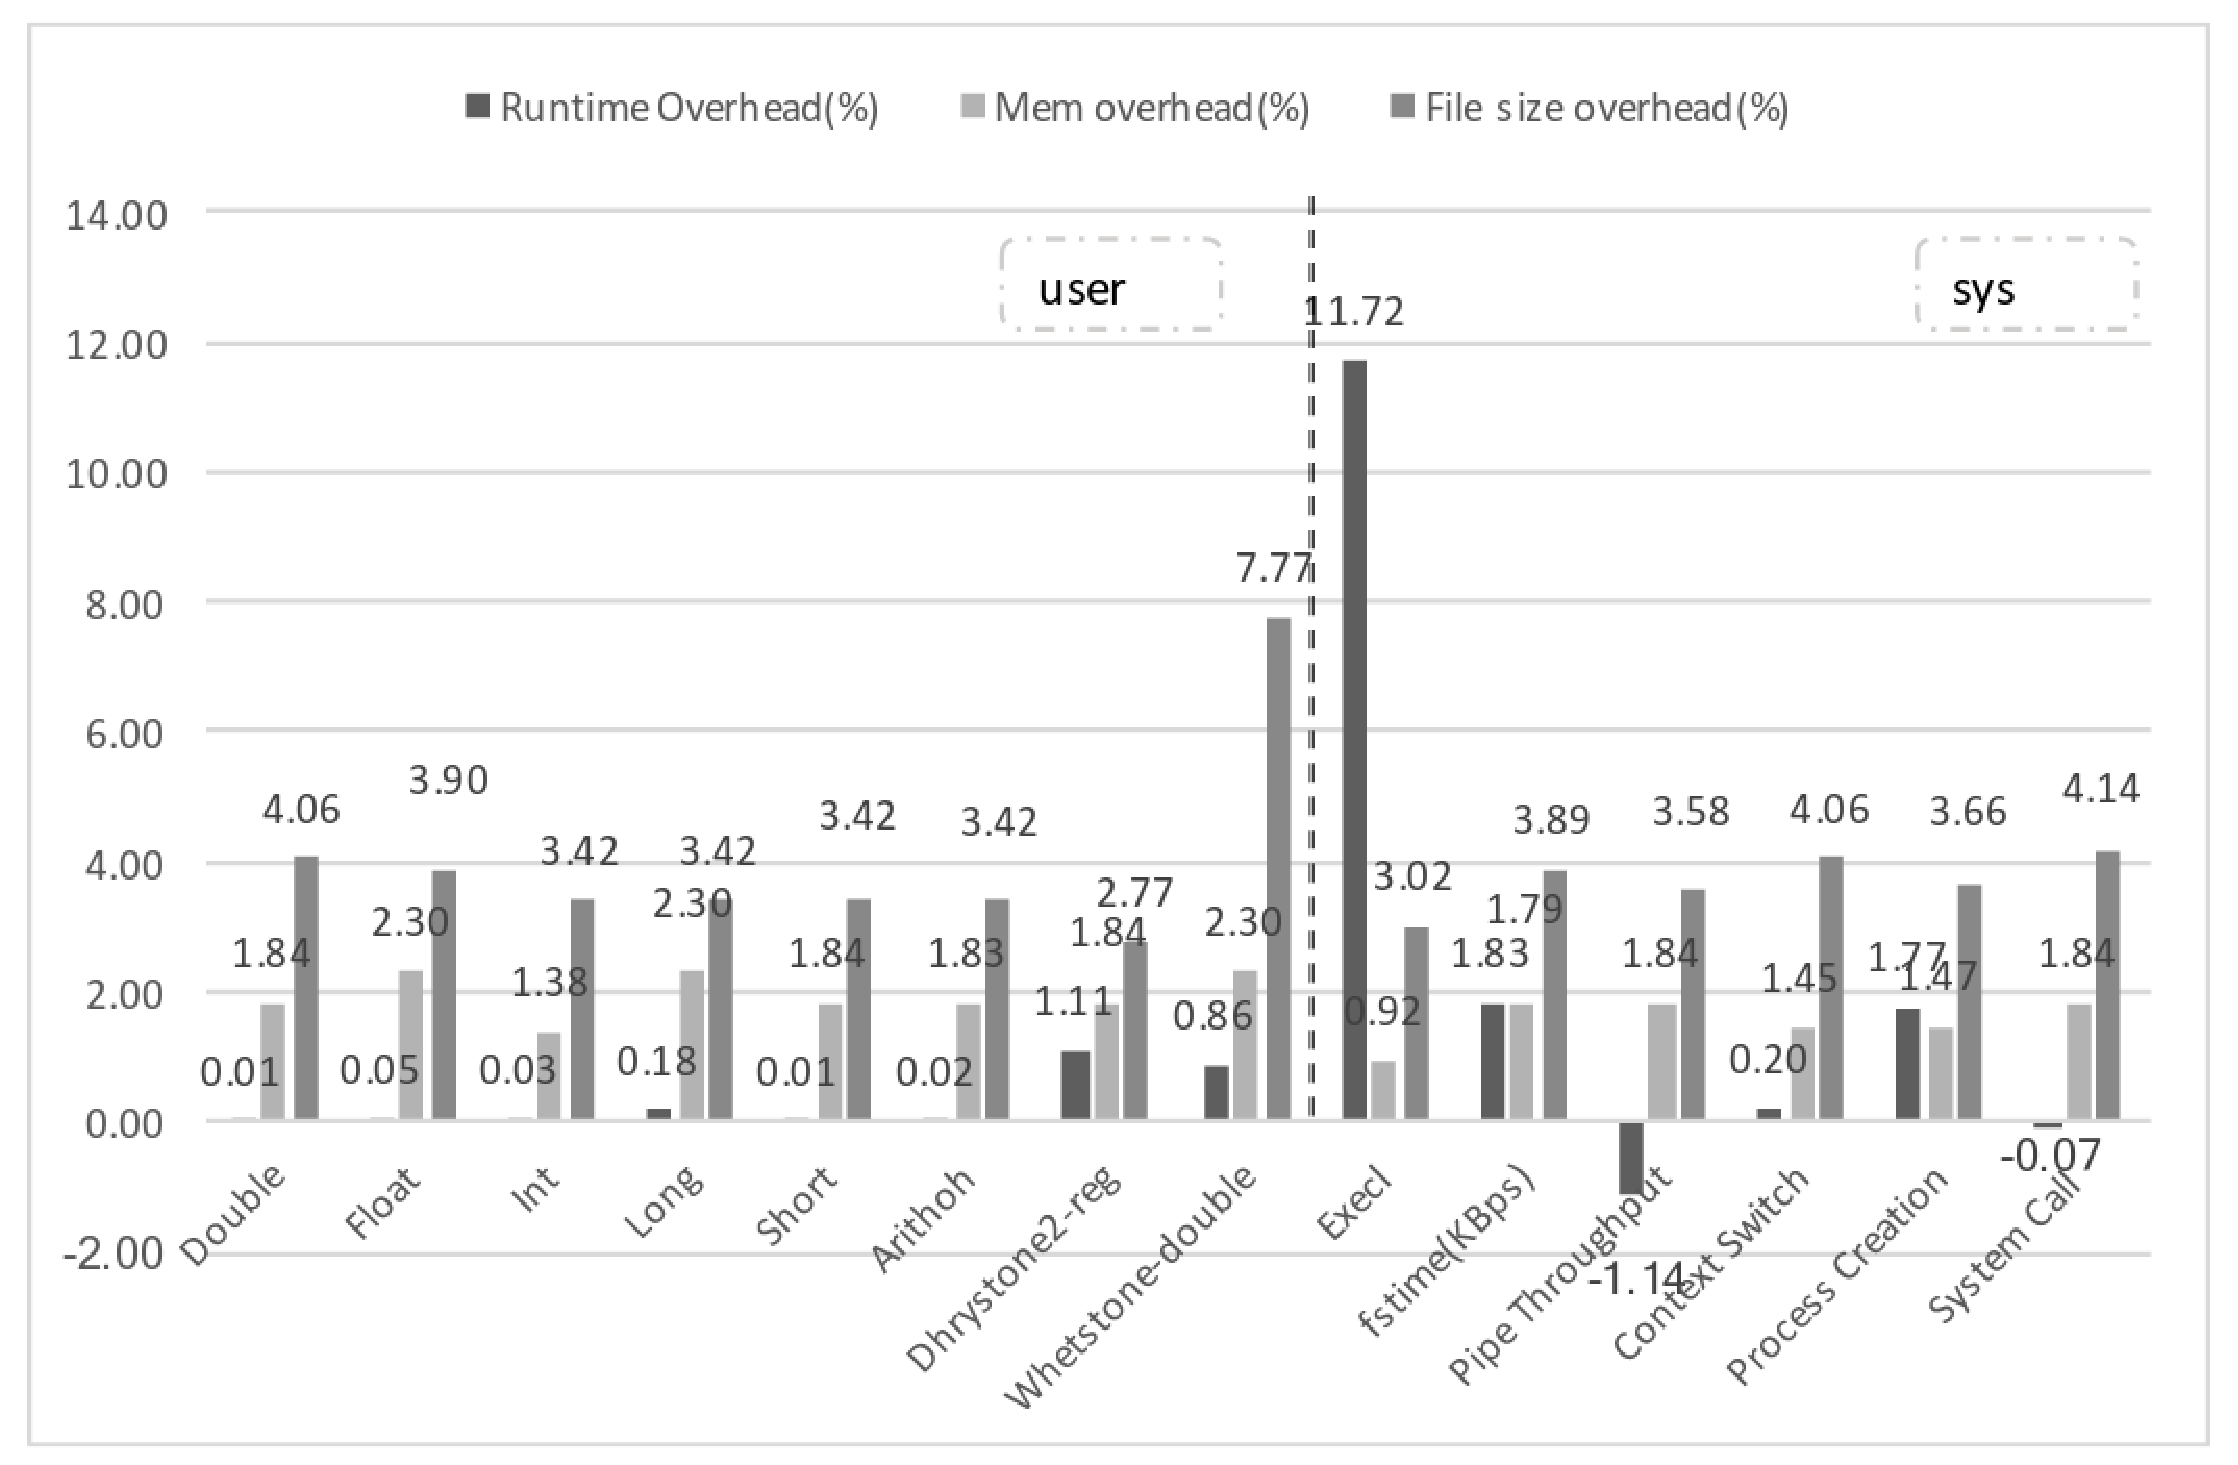
\includegraphics[width=1.0\linewidth]{figures/eval-performance.pdf}
\end{figure}
\end{columns}
\end{frame}

%------------------------------------------------

\section{Code Pointer?}
\begin{frame}
\frametitle{Code Pointer?}
\begin{itemize}
\item The address of next instruction after bl is stored on stack and visible to attacker
\item Function pointer or function address in .got are visible to attacker
\end{itemize}
\begin{figure}
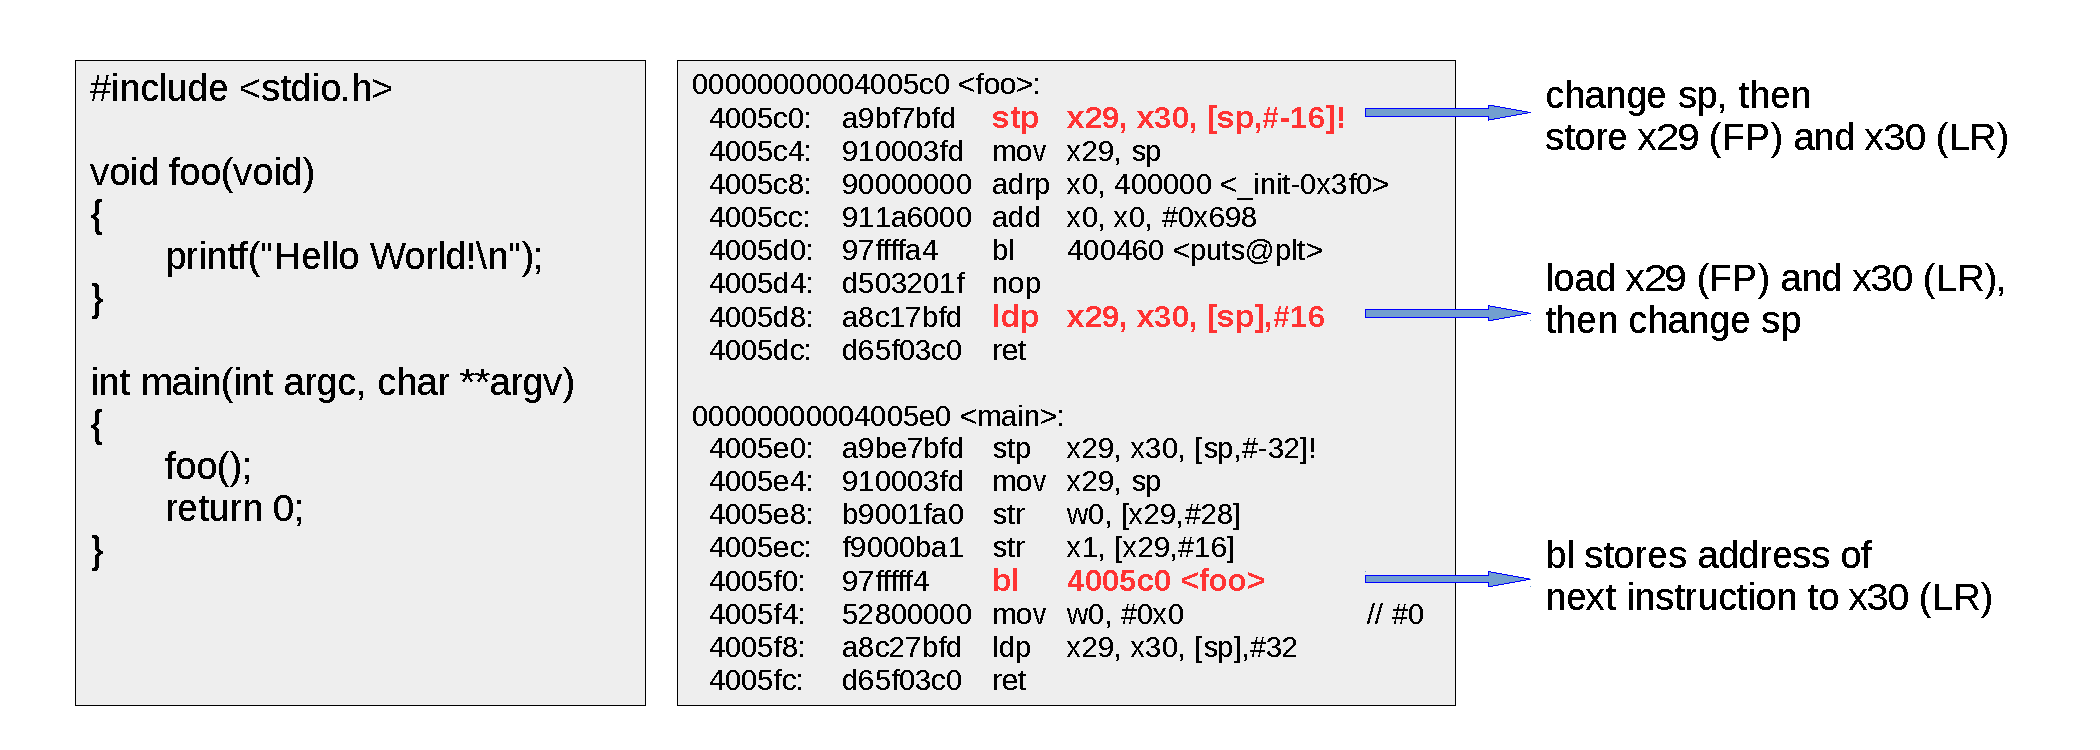
\includegraphics[width=1.0\linewidth]{figures/pointer.pdf}
\end{figure}
\end{frame}

%------------------------------------------------

\section{Interesting Paper/Link}
\begin{frame}
\frametitle{Interesting Paper/Link}
\begin{itemize}
\item 64-bit Linux Return-Oriented Programming. http://crypto.stanford.edu/$\sim$blynn/rop
\item ROPgadget: https://github.com/JonathanSalwan/ROPgadget
\item Practical Code Randomization Resilient to Memory Disclosure. IEEE S \& P 2015
\item Control Flow Integrity for COTS Binaries. USENIX Security 2013
\item SoK: Eternal War in Memory. IEEE S \& P 2013
\item http://shell-storm.org
\item Control-Flow Integrity. CCS 2005
\end{itemize}
\end{frame}

%------------------------------------------------

\section{Take-Home Message}
\begin{frame}
\frametitle{Take-Home Message}
\begin{columns}[c]
\column{.75\textwidth}
\begin{itemize}
\visible<1->{\item Shellcode injection and execution are not prerequisite for ROP}
\visible<2->{\item Fine-grained ASLR cannot defend JIT-ROP attack}
\visible<3->{\item Direct memory disclosure and indirect memory disclosure}
\visible<4->{\item XOM is supported by Intel EPT and AArch64 userspace}
\visible<5->{\item Code-data separation is possible for AArch64 COTS binary}
\end{itemize}
\column{.25\textwidth}
\begin{center}
\begin{figure}

\includegraphics[width=.8\linewidth]{figures/home.pdf}
\end{figure}
\end{center}
\end{columns}
\end{frame}

%\begin{frame}
%\Huge{\centerline{The End}}
%\end{frame}

%----------------------------------------------------------------------------------------

\end{document} 
